\chapter{Annex}


\begin{figure}[h]
  \centering
  \subfigure[Rendering Picture]{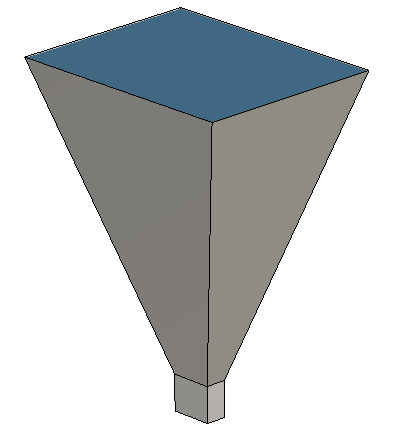
\includegraphics[height=6cm]{Antennas/Horn.png}}
  \centering
  \subfigure[Pattern]{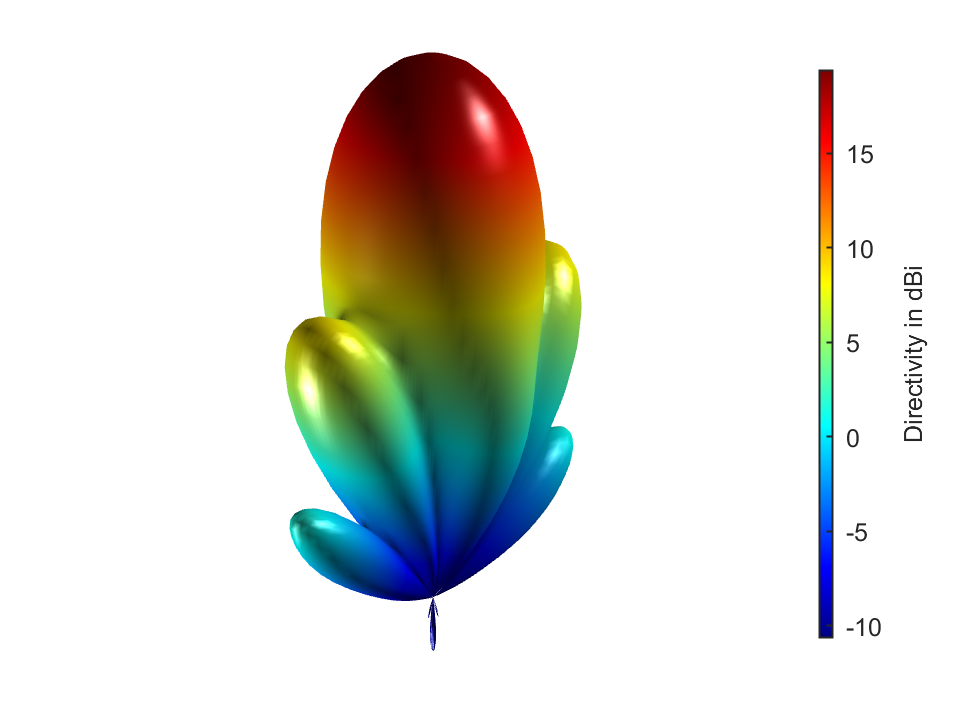
\includegraphics[height=6cm]{Antennas/horn_3D.png}}
\caption{$\SI{20}{\decibel}$ SGH}
\label{fig:hornpro}
\end{figure}

\begin{figure}[h]
  \centering
  \subfigure[Rendering Picture]{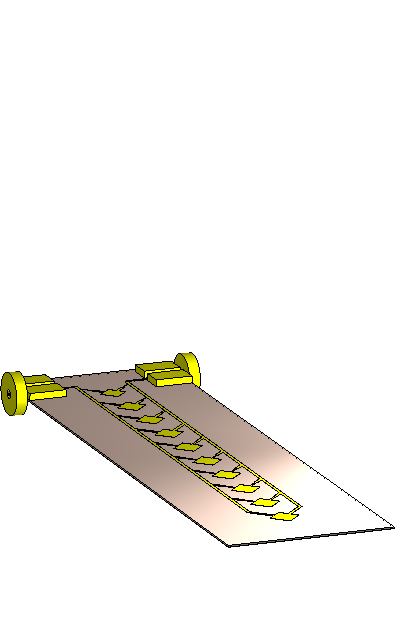
\includegraphics[height=6cm]{Antennas/10x1-array.png}}
  \centering
  \subfigure[Pattern]{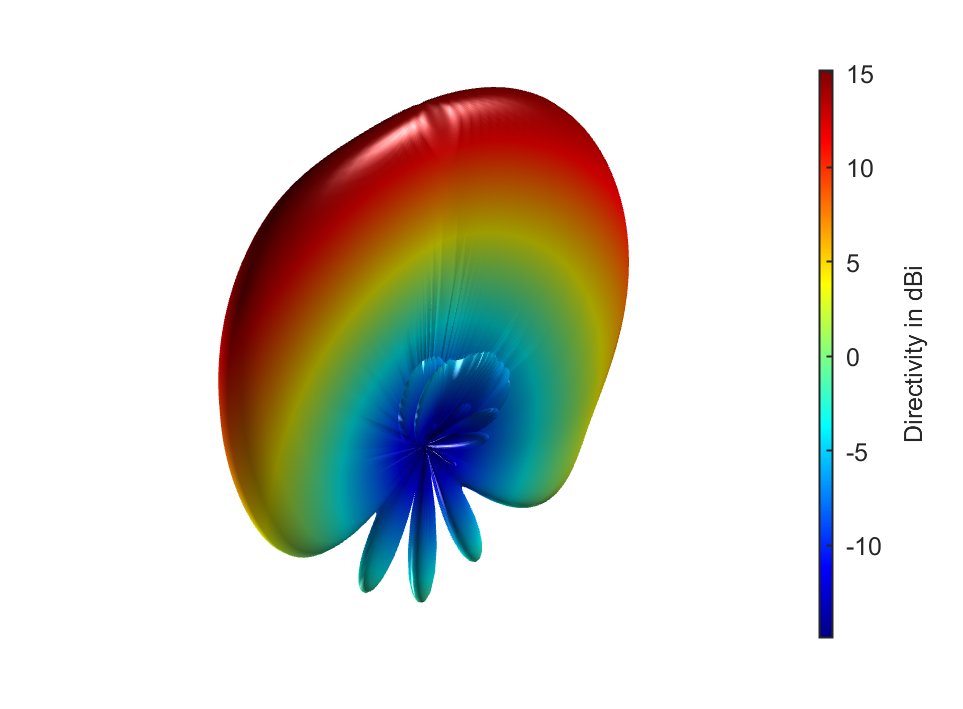
\includegraphics[height=6cm]{Antennas/10x1-array_3D.png}}
\caption{10x1 Patch array developed in \cite{7481205}}
\label{fig:10x1a}
\end{figure}

\begin{figure}[h]
  \centering
  \subfigure[Rendering Picture]{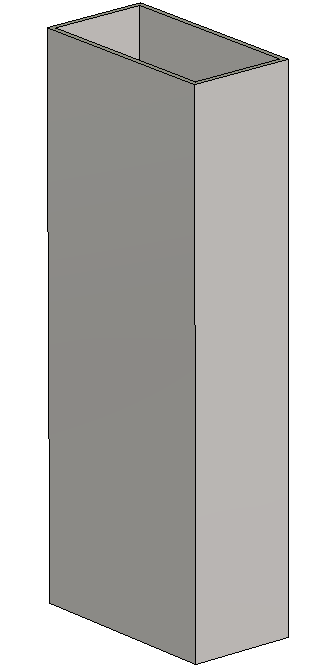
\includegraphics[height=6cm]{Antennas/OEWG.png}}
  \centering
  \subfigure[Pattern]{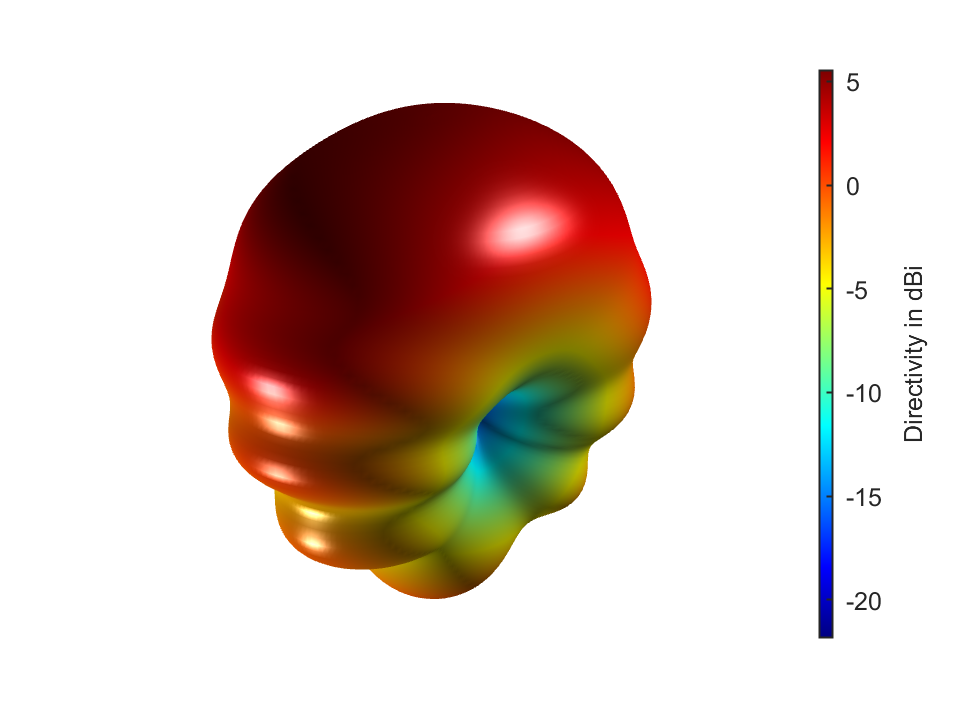
\includegraphics[height=6cm]{Antennas/oewg_3D.png}}
\caption{OEWG}
\label{fig:oewgpro}
\end{figure}

\begin{figure}[h]
  \centering
  \subfigure[Rendering Picture]{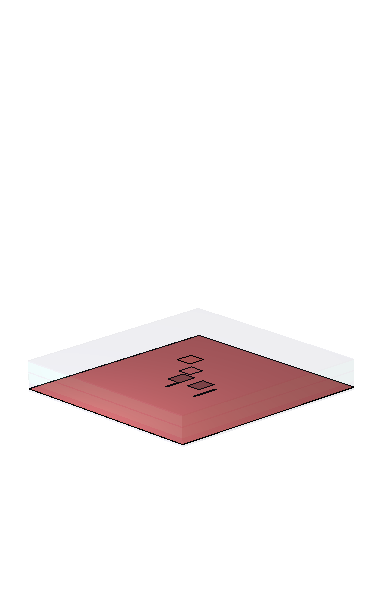
\includegraphics[height=6cm]{Antennas/patch.png}}
  \centering
  \subfigure[Pattern]{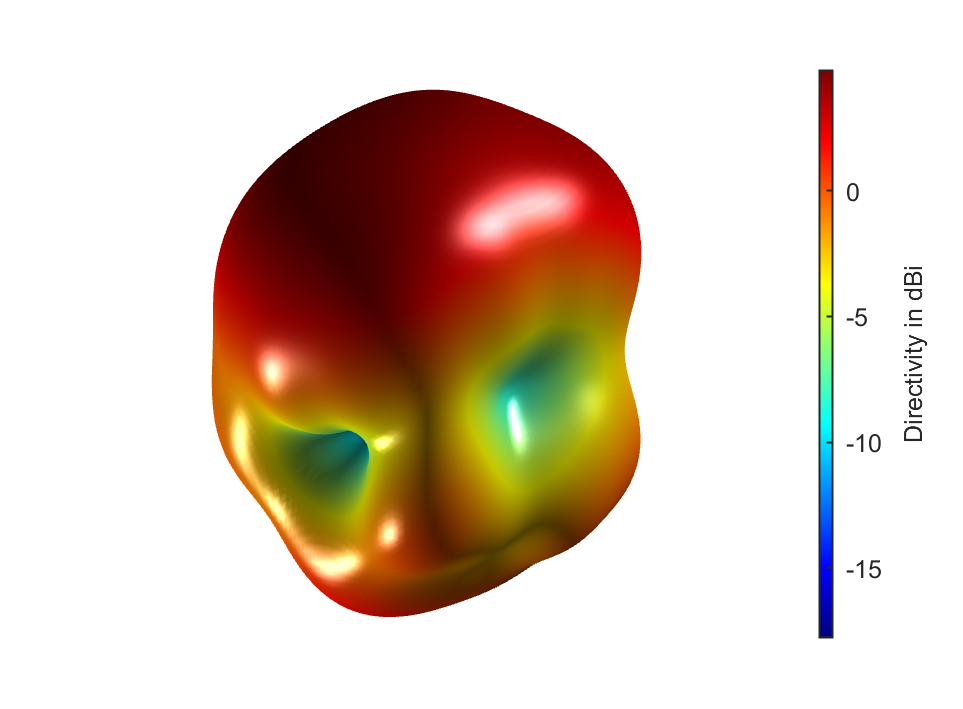
\includegraphics[height=6cm]{Antennas/patch_3D.png}}
\caption{R\&{}S experimental patch antenna}
\label{fig:patchpro}
\end{figure}


\begin{figure}[h]
  \centering
  \subfigure[High Gain Horn]{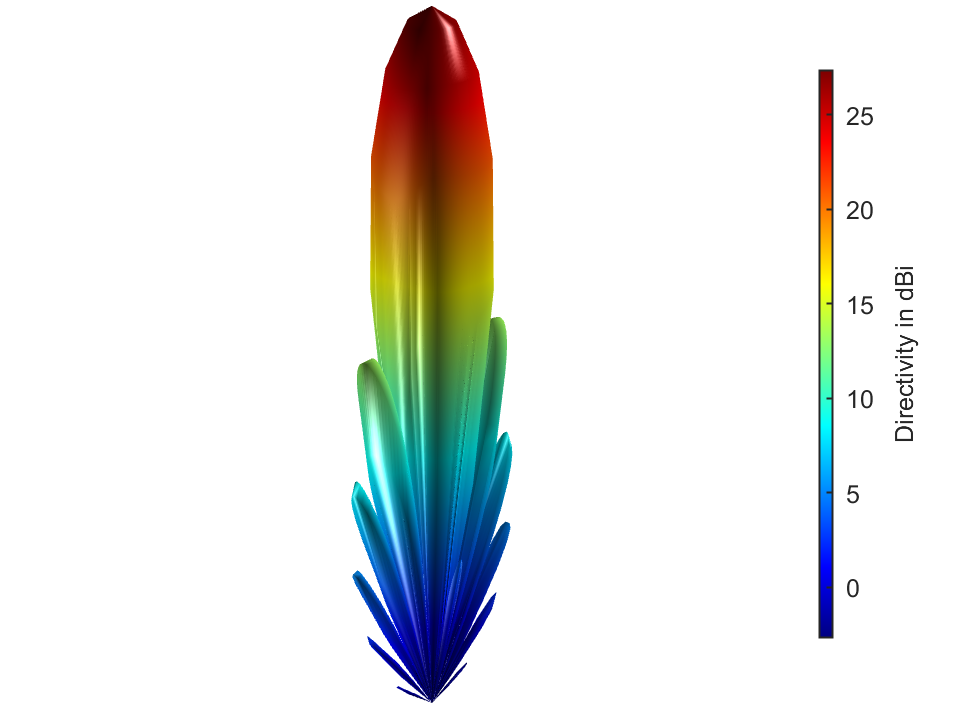
\includegraphics[width=0.49\textwidth]{Antennas/26dBHorn_3D.png}}
  \centering
  \subfigure[2x2 $\SI{20}{\decibel}$ SGH Array]{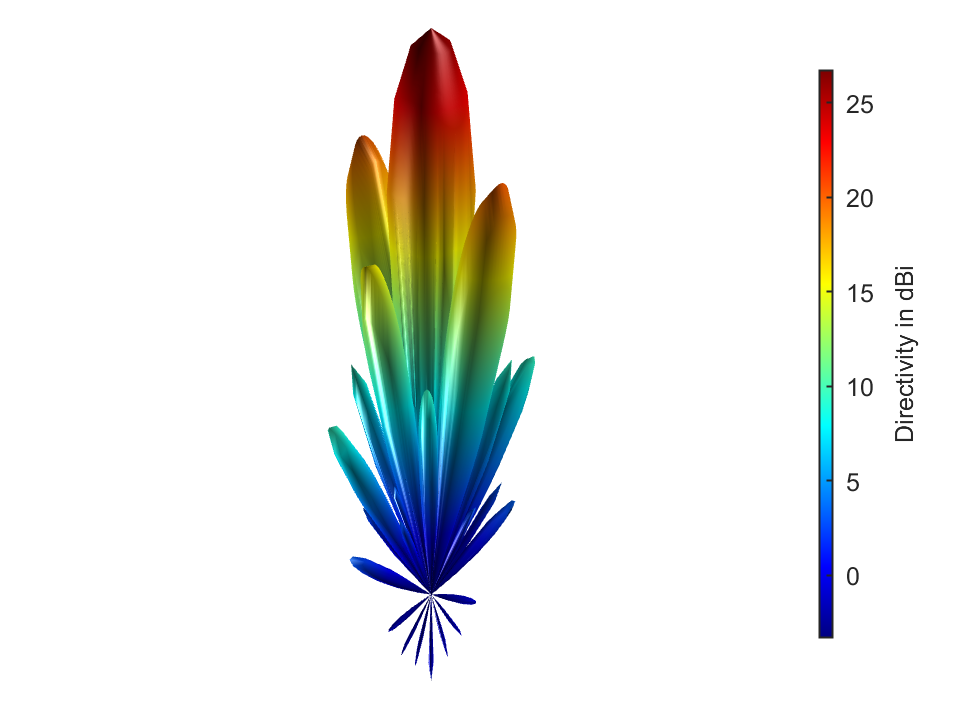
\includegraphics[width=0.49\textwidth]{Antennas/HornArray_3D.png}}
  \centering
  \subfigure[$\sfrac{\lambda}{2}$ Dipole]{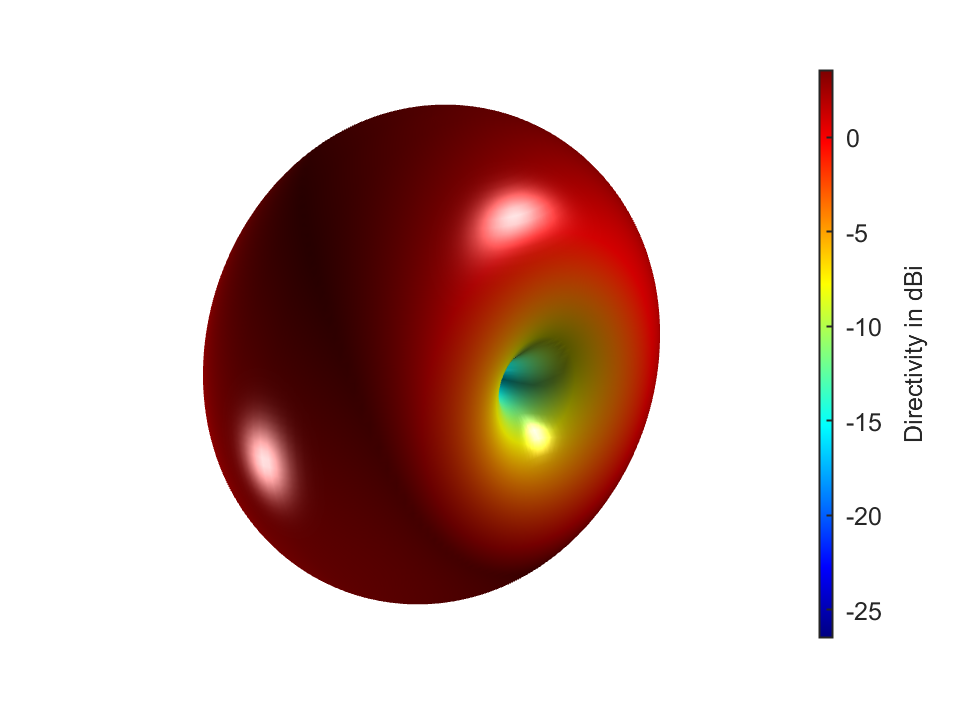
\includegraphics[width=0.49\textwidth]{Antennas/dipole_3D.png}}
  \centering
  \subfigure[Hertz Dipole]{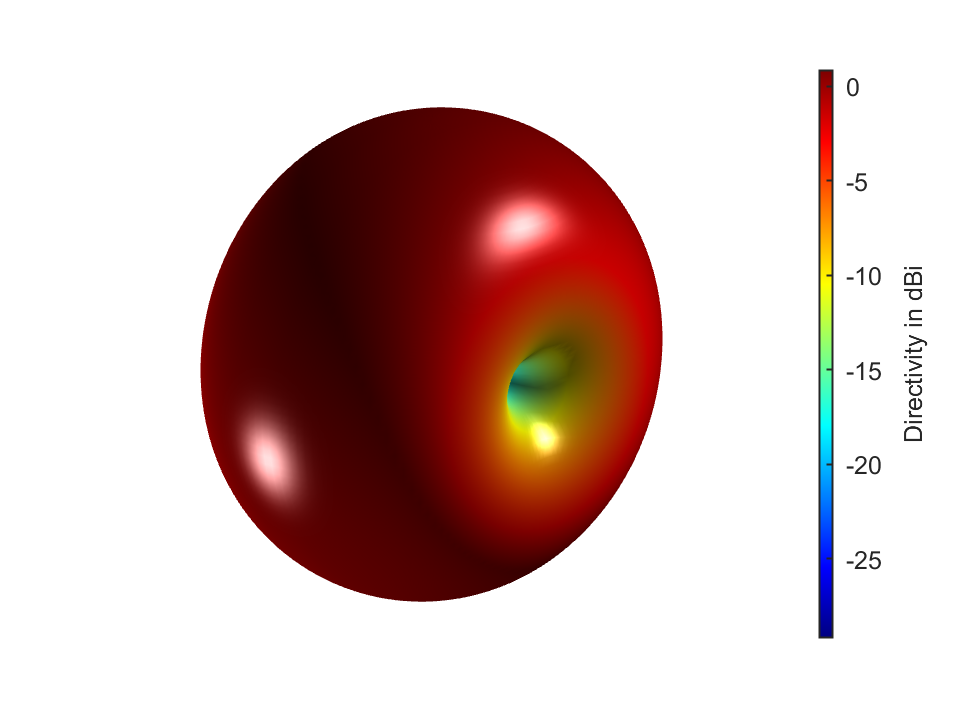
\includegraphics[width=0.49\textwidth]{Antennas/dipole-hertz_3D.png}}
\caption{Patterns of other antennas}
\label{fig:othera}
\end{figure}

\begin{figure}
\centering
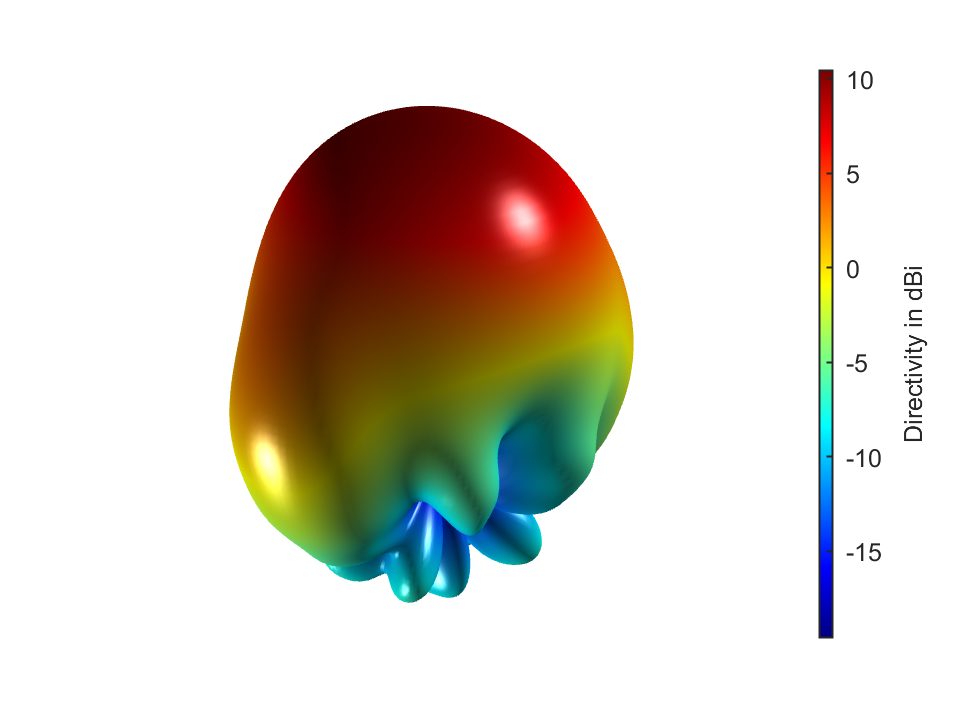
\includegraphics[width=0.49\textwidth]{Antennas/OEWG-Imp1_3D.png}
\caption{Antenna pattern of OEWG implementation one}
\label{fig:oewgimpone}
\end{figure}

\begin{figure}
  \centering
  \subfigure[Constant Step Size Polar Coordinates]{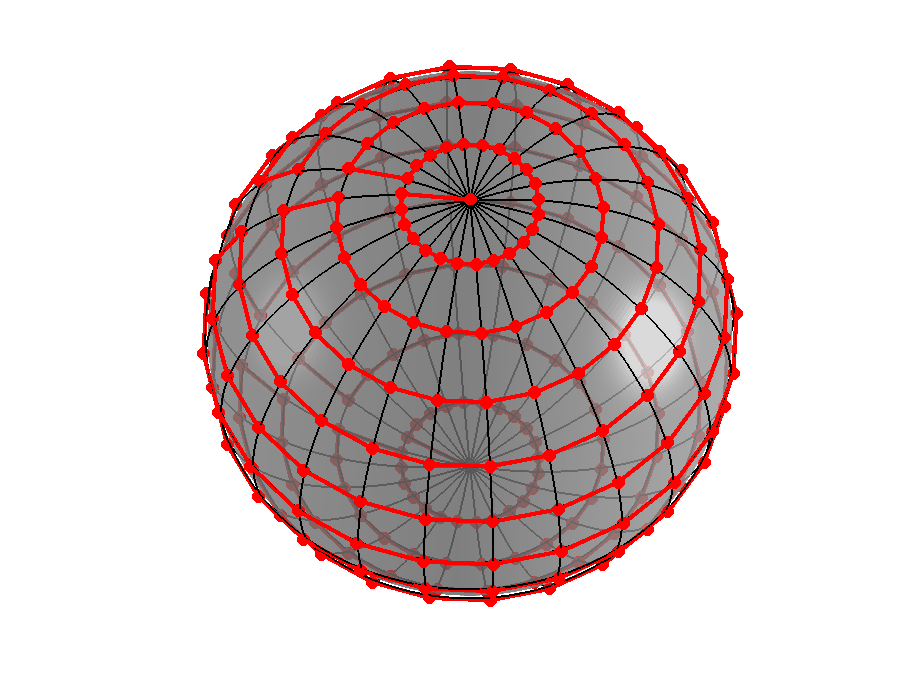
\includegraphics[width=0.49\textwidth]{Matlab/GridCoStPolar.eps}}
  \centering
  \subfigure[Constant Step Size Cartesian Coordinates]{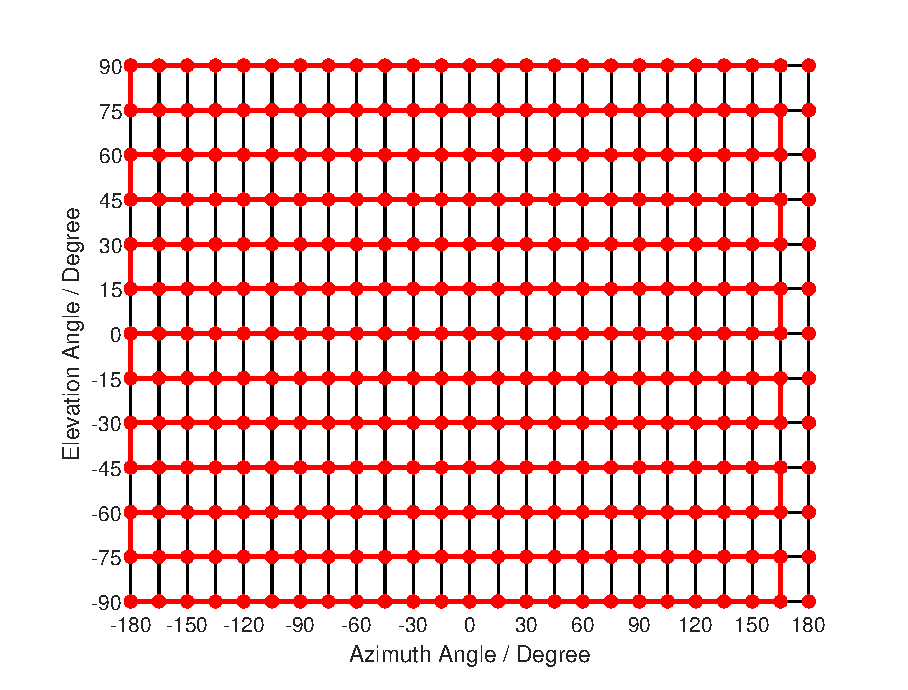
\includegraphics[width=0.49\textwidth]{Matlab/GridCoStCart.eps}}
  \centering
  \subfigure[Constant Step Size sinTF Polar Coordinates]{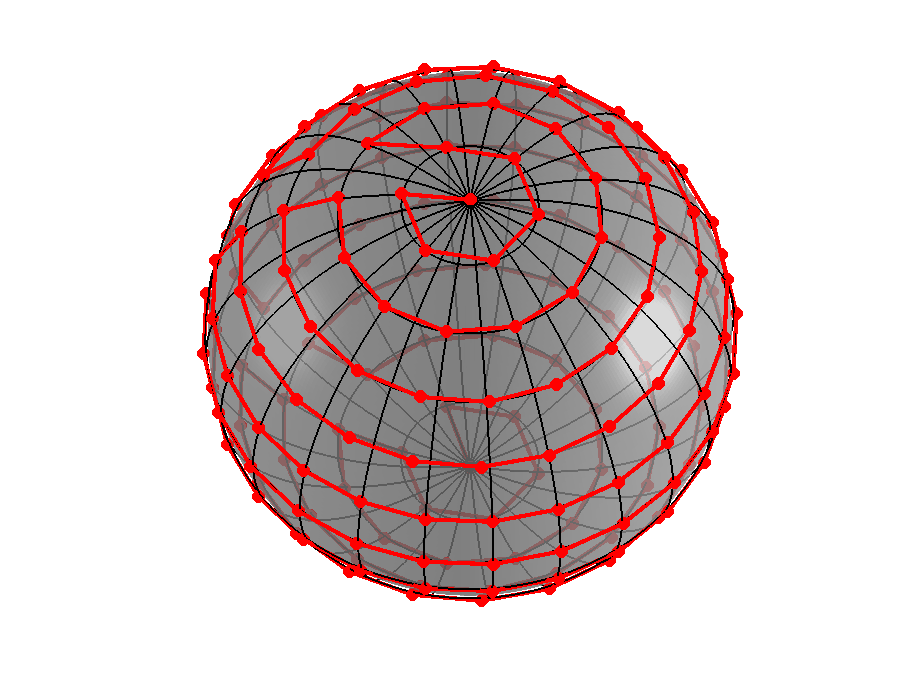
\includegraphics[width=0.49\textwidth]{Matlab/GridCoStSinPolar.eps}}
  \centering
  \subfigure[Constant Step Size sinTF Cartesian Coordinates]{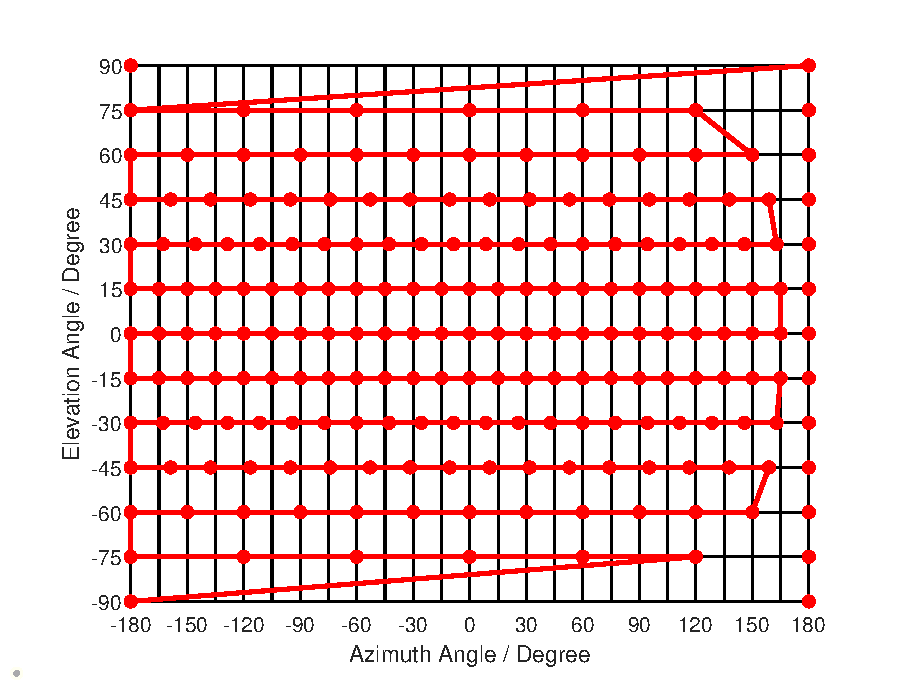
\includegraphics[width=0.49\textwidth]{Matlab/GridCoStSinCart.eps}}
  \centering
  \subfigure[Constant Density Polar Coordinates]{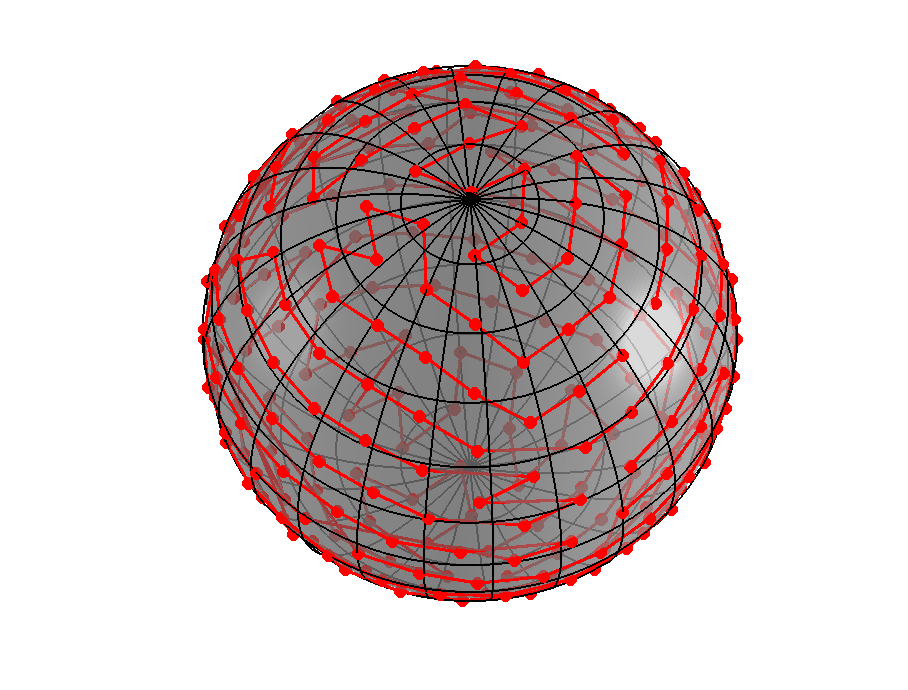
\includegraphics[width=0.49\textwidth]{Matlab/GridCoDePolar.eps}}
  \centering
  \subfigure[Constant Density Cartesian Coordinates]{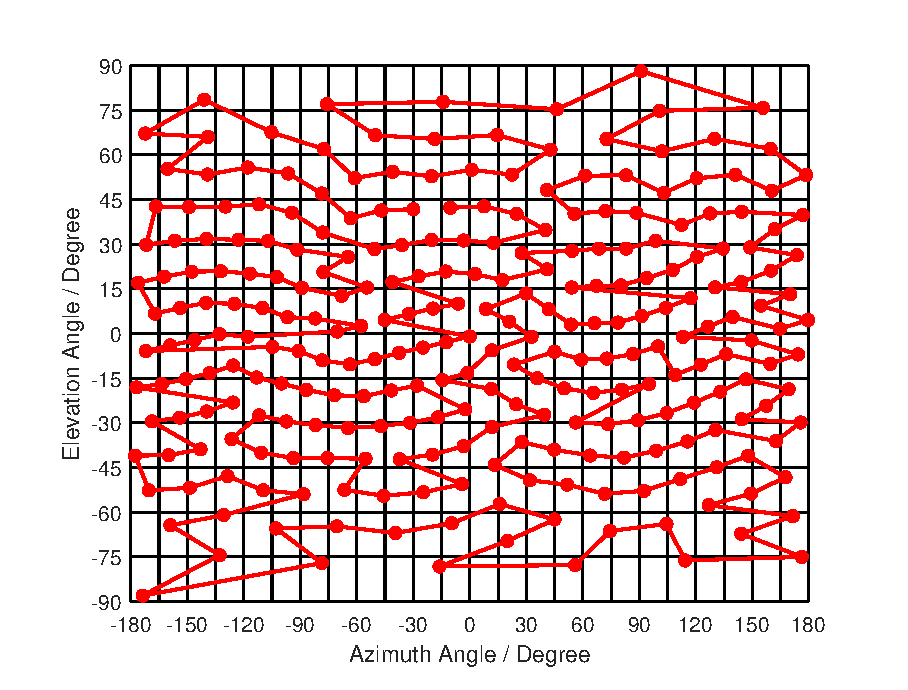
\includegraphics[width=0.49\textwidth]{Matlab/GridCoDeCart.eps}}
\caption{Different spherical sampling grids in comparison}
\label{fig:gridcomp}
\end{figure}


\begin{figure}
  \centering
  \subfigure[Two elements: Pattern]{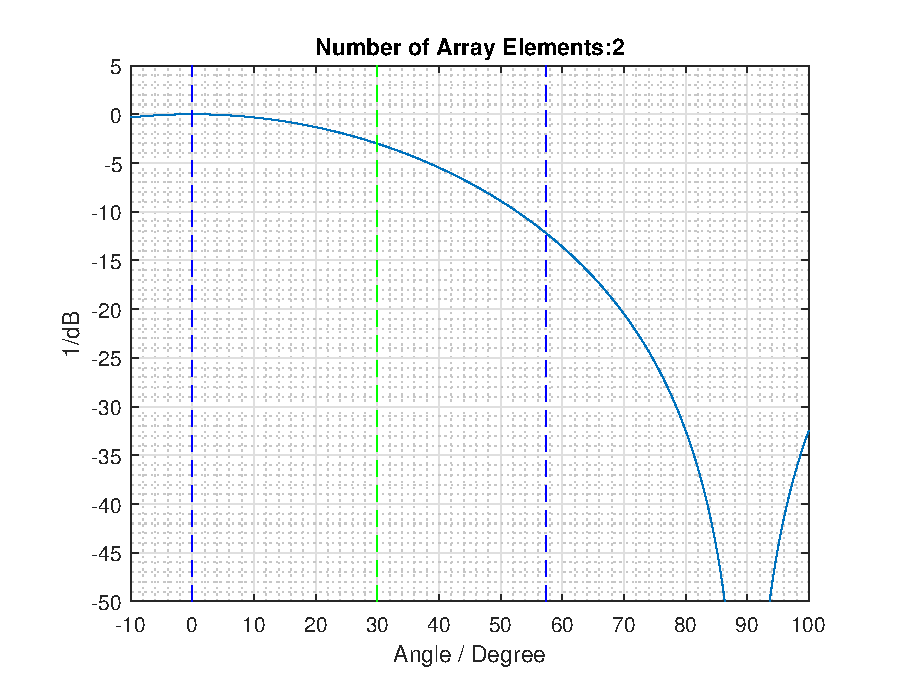
\includegraphics[width=0.45\textwidth]{Matlab/NoNumEl2.eps}}
  \centering
  \subfigure[Two elements: Mode spectra]{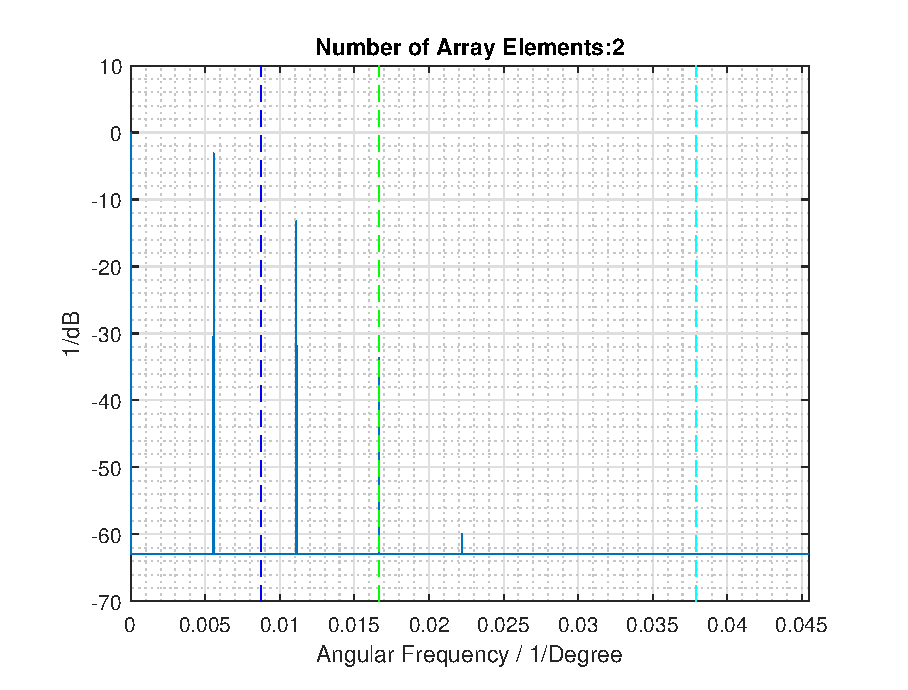
\includegraphics[width=0.45\textwidth]{Matlab/SpNumEl2.eps}}
  \centering
  \subfigure[Six elements: Pattern]{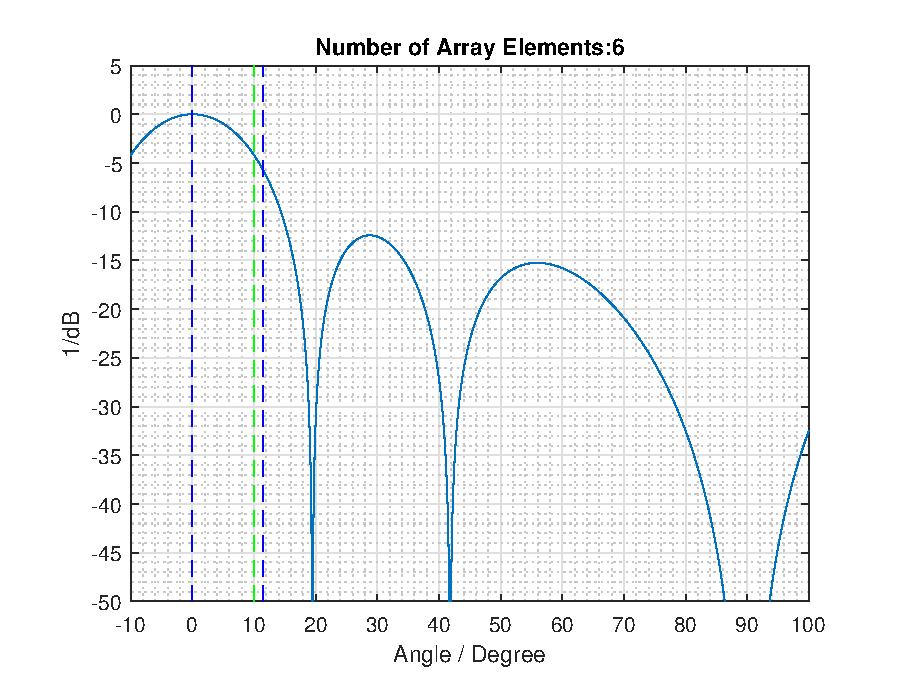
\includegraphics[width=0.45\textwidth]{Matlab/NoNumEl6.eps}}
  \centering
  \subfigure[Six elements: Mode spectra]{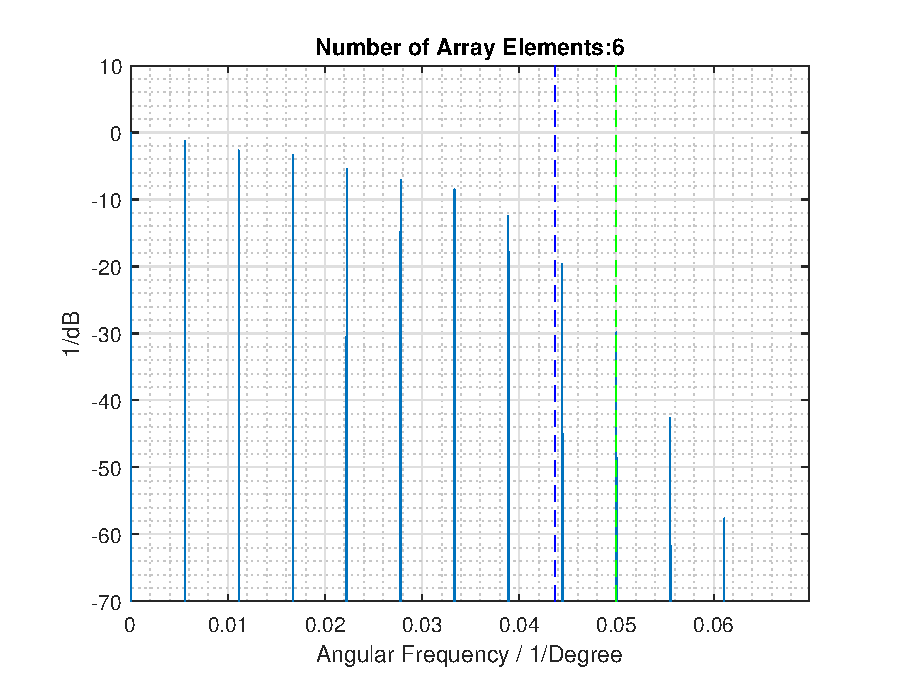
\includegraphics[width=0.45\textwidth]{Matlab/SpNumEl6.eps}}
  \centering
  \subfigure[100 elements: Pattern]{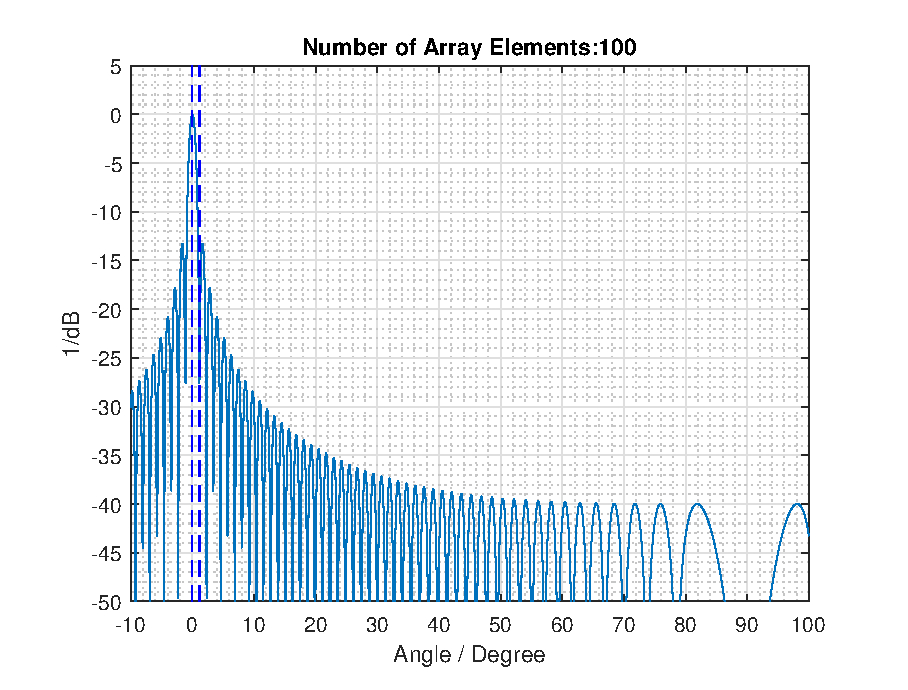
\includegraphics[width=0.45\textwidth]{Matlab/NoNumEl100.eps}}
  \centering
  \subfigure[100 elements: Mode spectra]{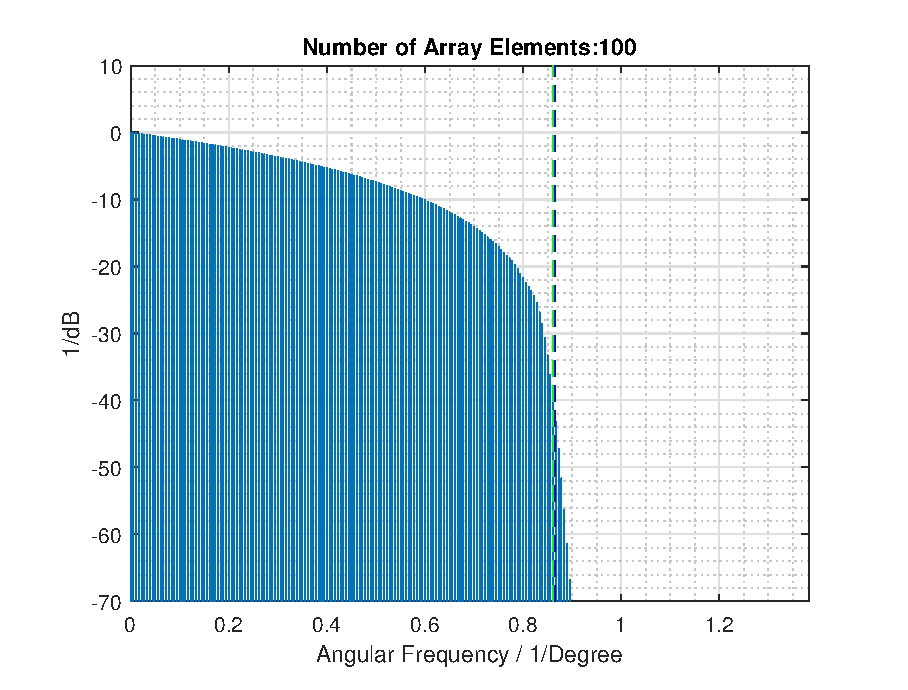
\includegraphics[width=0.45\textwidth]{Matlab/SpNumEl100.eps}}
\caption{Pattern of $N$-element $\sfrac{\lambda}{2}$-spacing}
\label{fig:evolvpattern}
\end{figure}

\begin{figure}
\centering
  \centering
  \subfigure[E-Field]{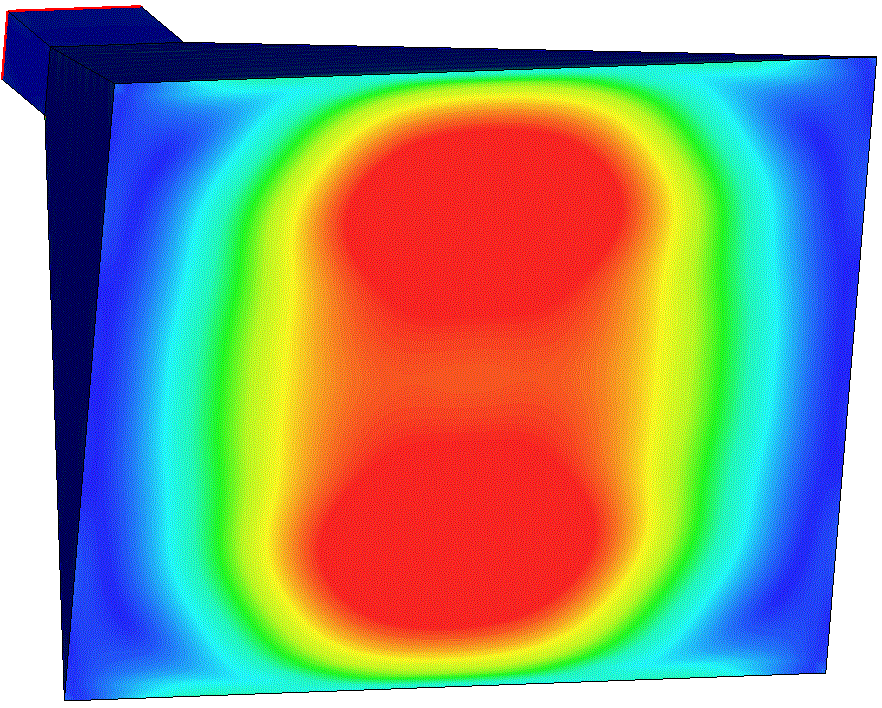
\includegraphics[width=0.49\textwidth]{horn_e_Field_FrontView.png}}
  \centering
  \subfigure[H-Field]{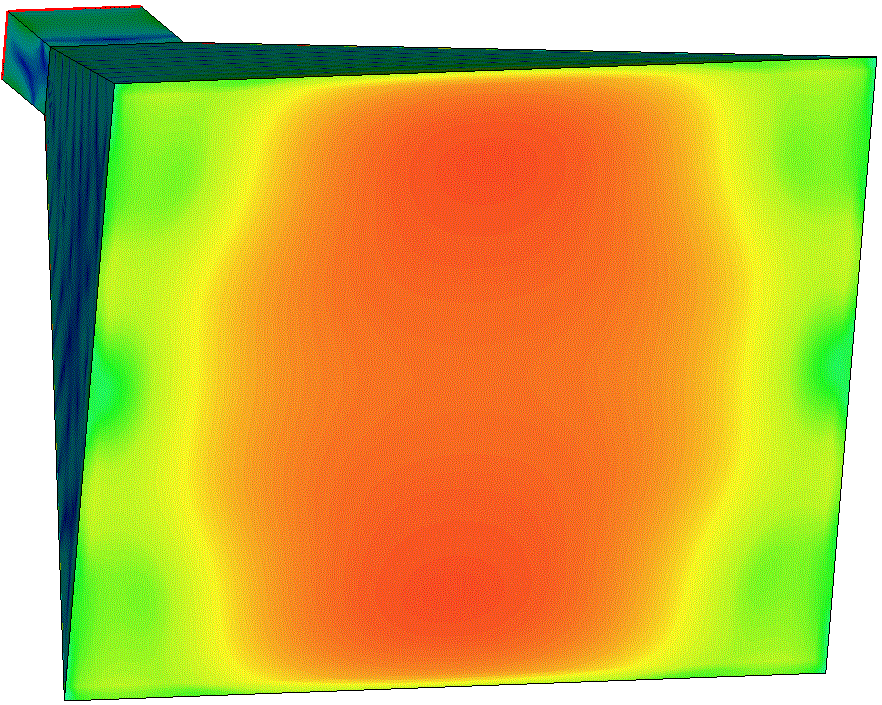
\includegraphics[width=0.49\textwidth]{horn_h_Field_FrontView.png}}
\caption{Field distribution on the aperture of a $\SI{20}{\decibel}$ SGH at $\SI{28}{\giga\hertz}$}
\label{fig:fielddist}
\end{figure}

\begin{figure}
\centering
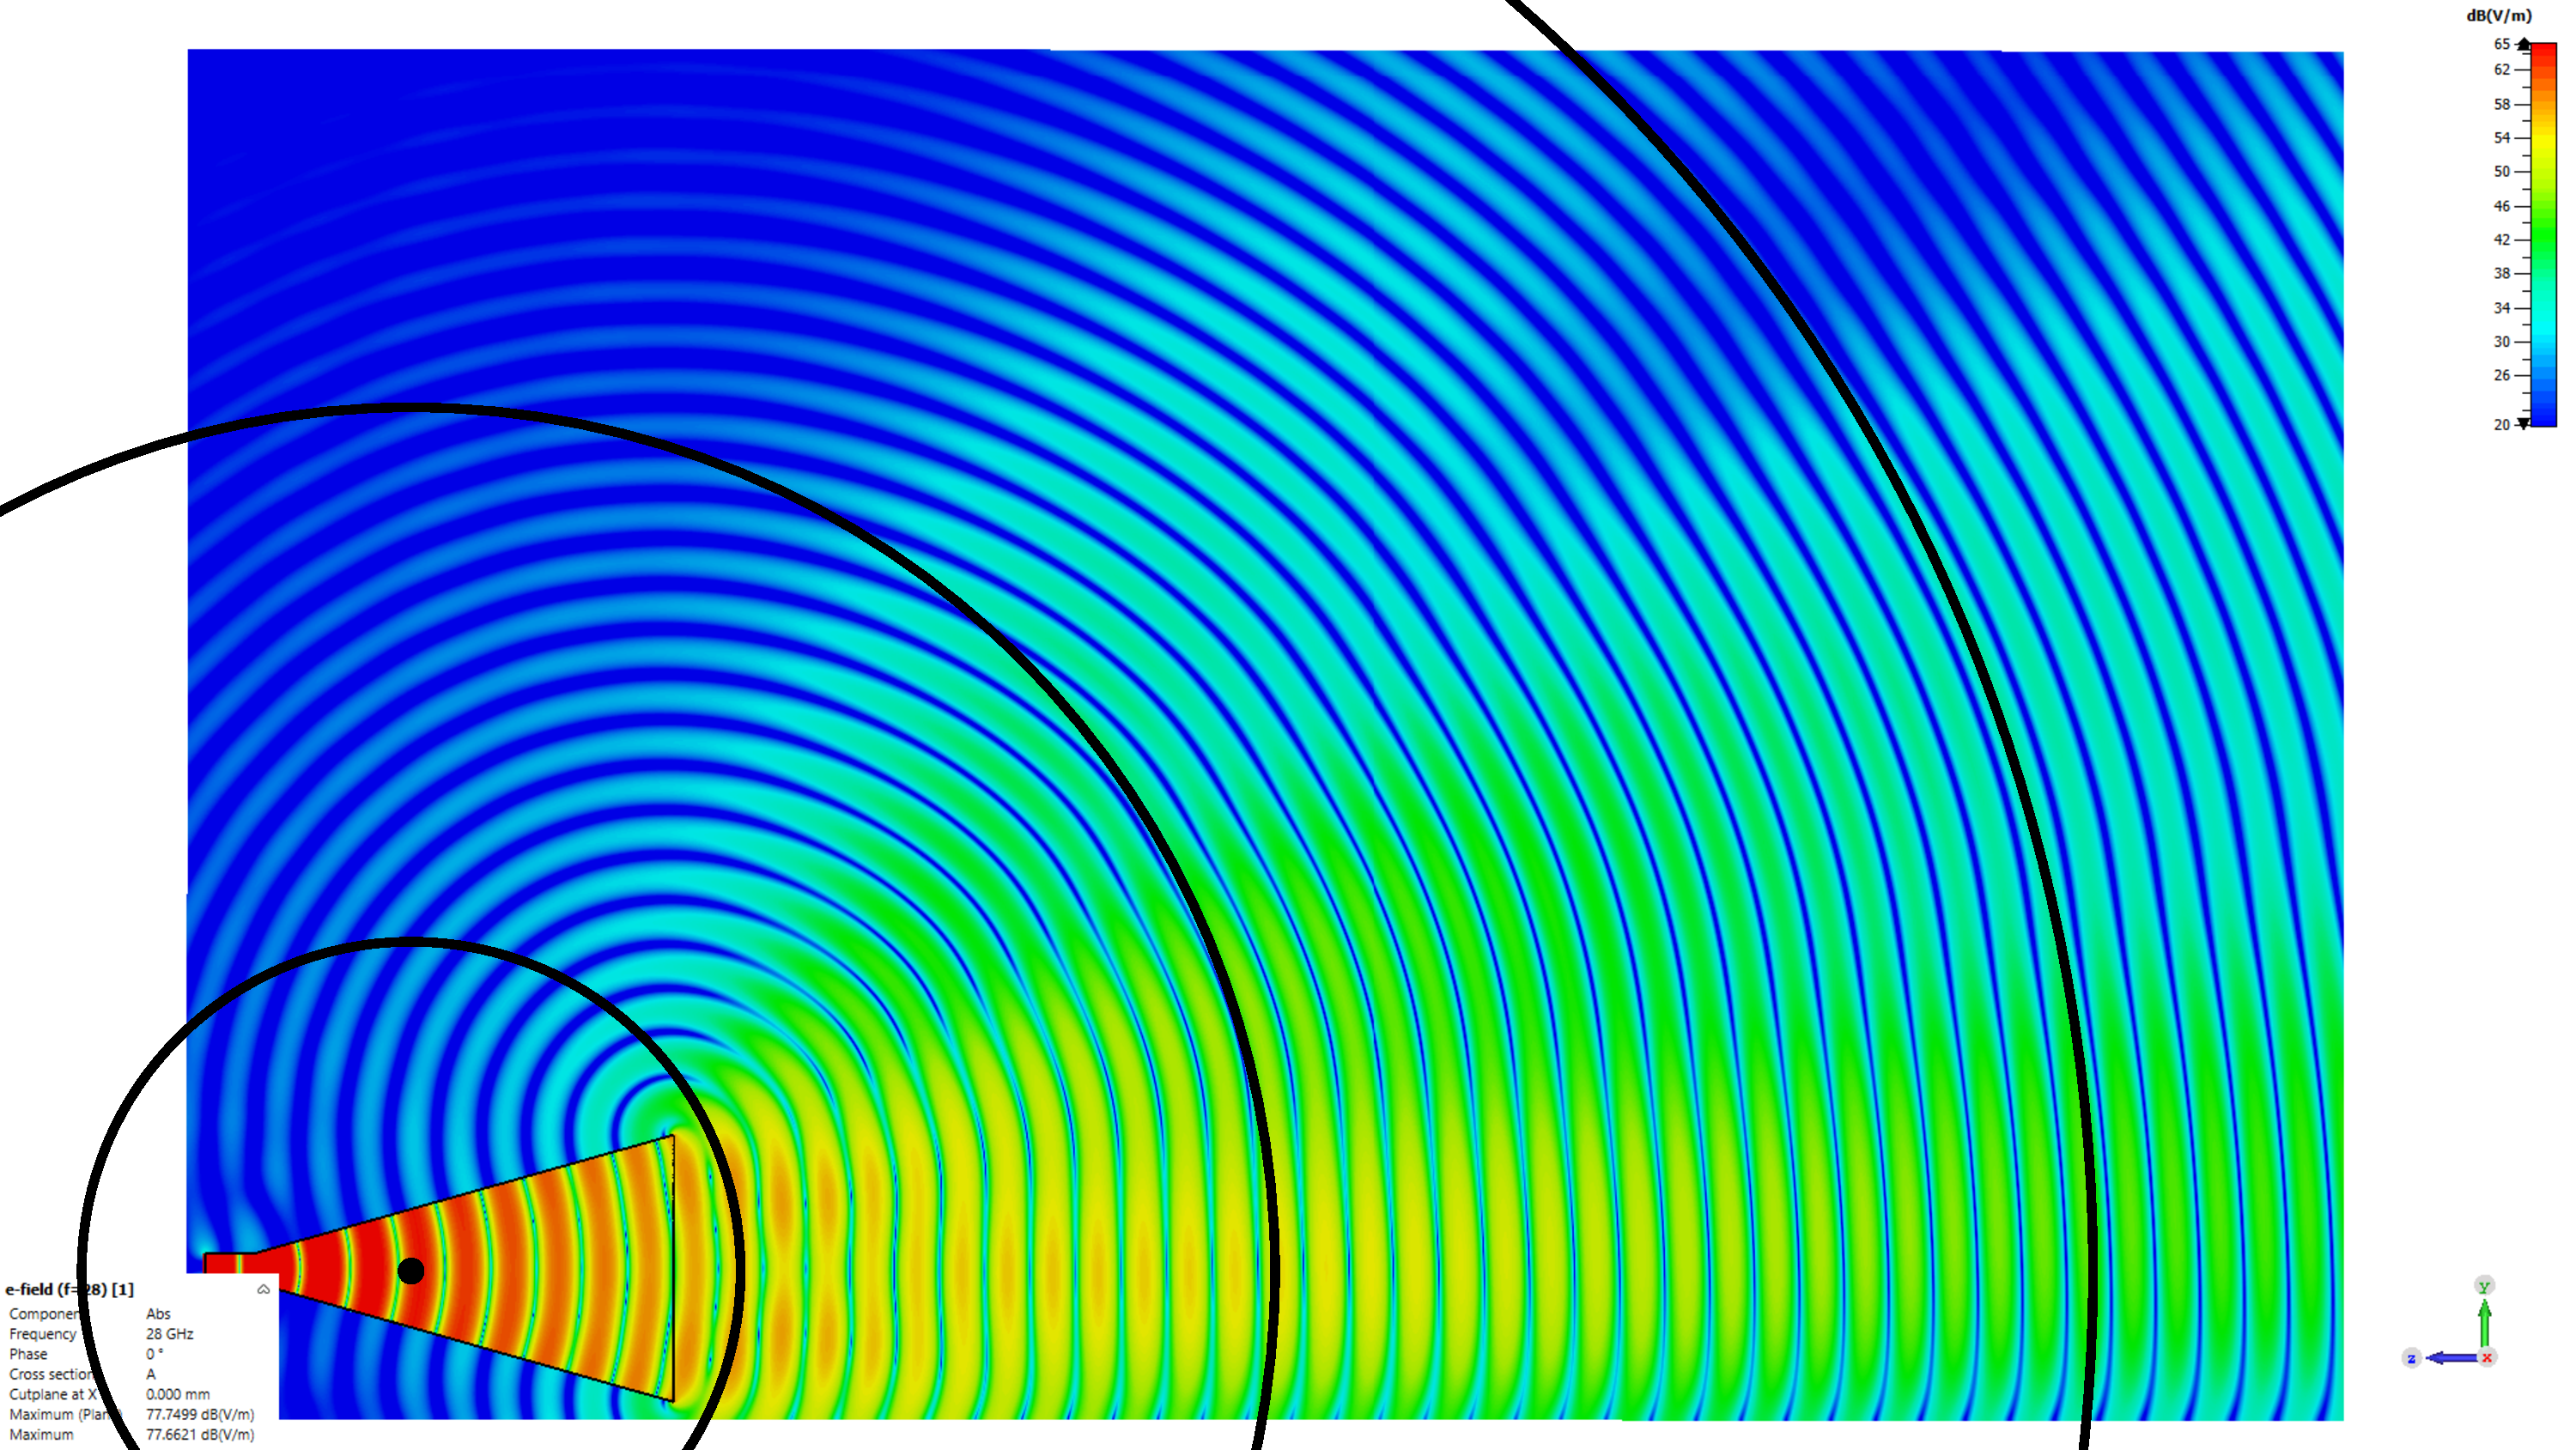
\includegraphics[width=1.5\textwidth , angle=90]{Horn-ef-Field-Region.pdf}
\caption{E-Field of a SGH in E-Plane}
\label{fig:eplaneef}
\end{figure}
\begin{figure}
\centering
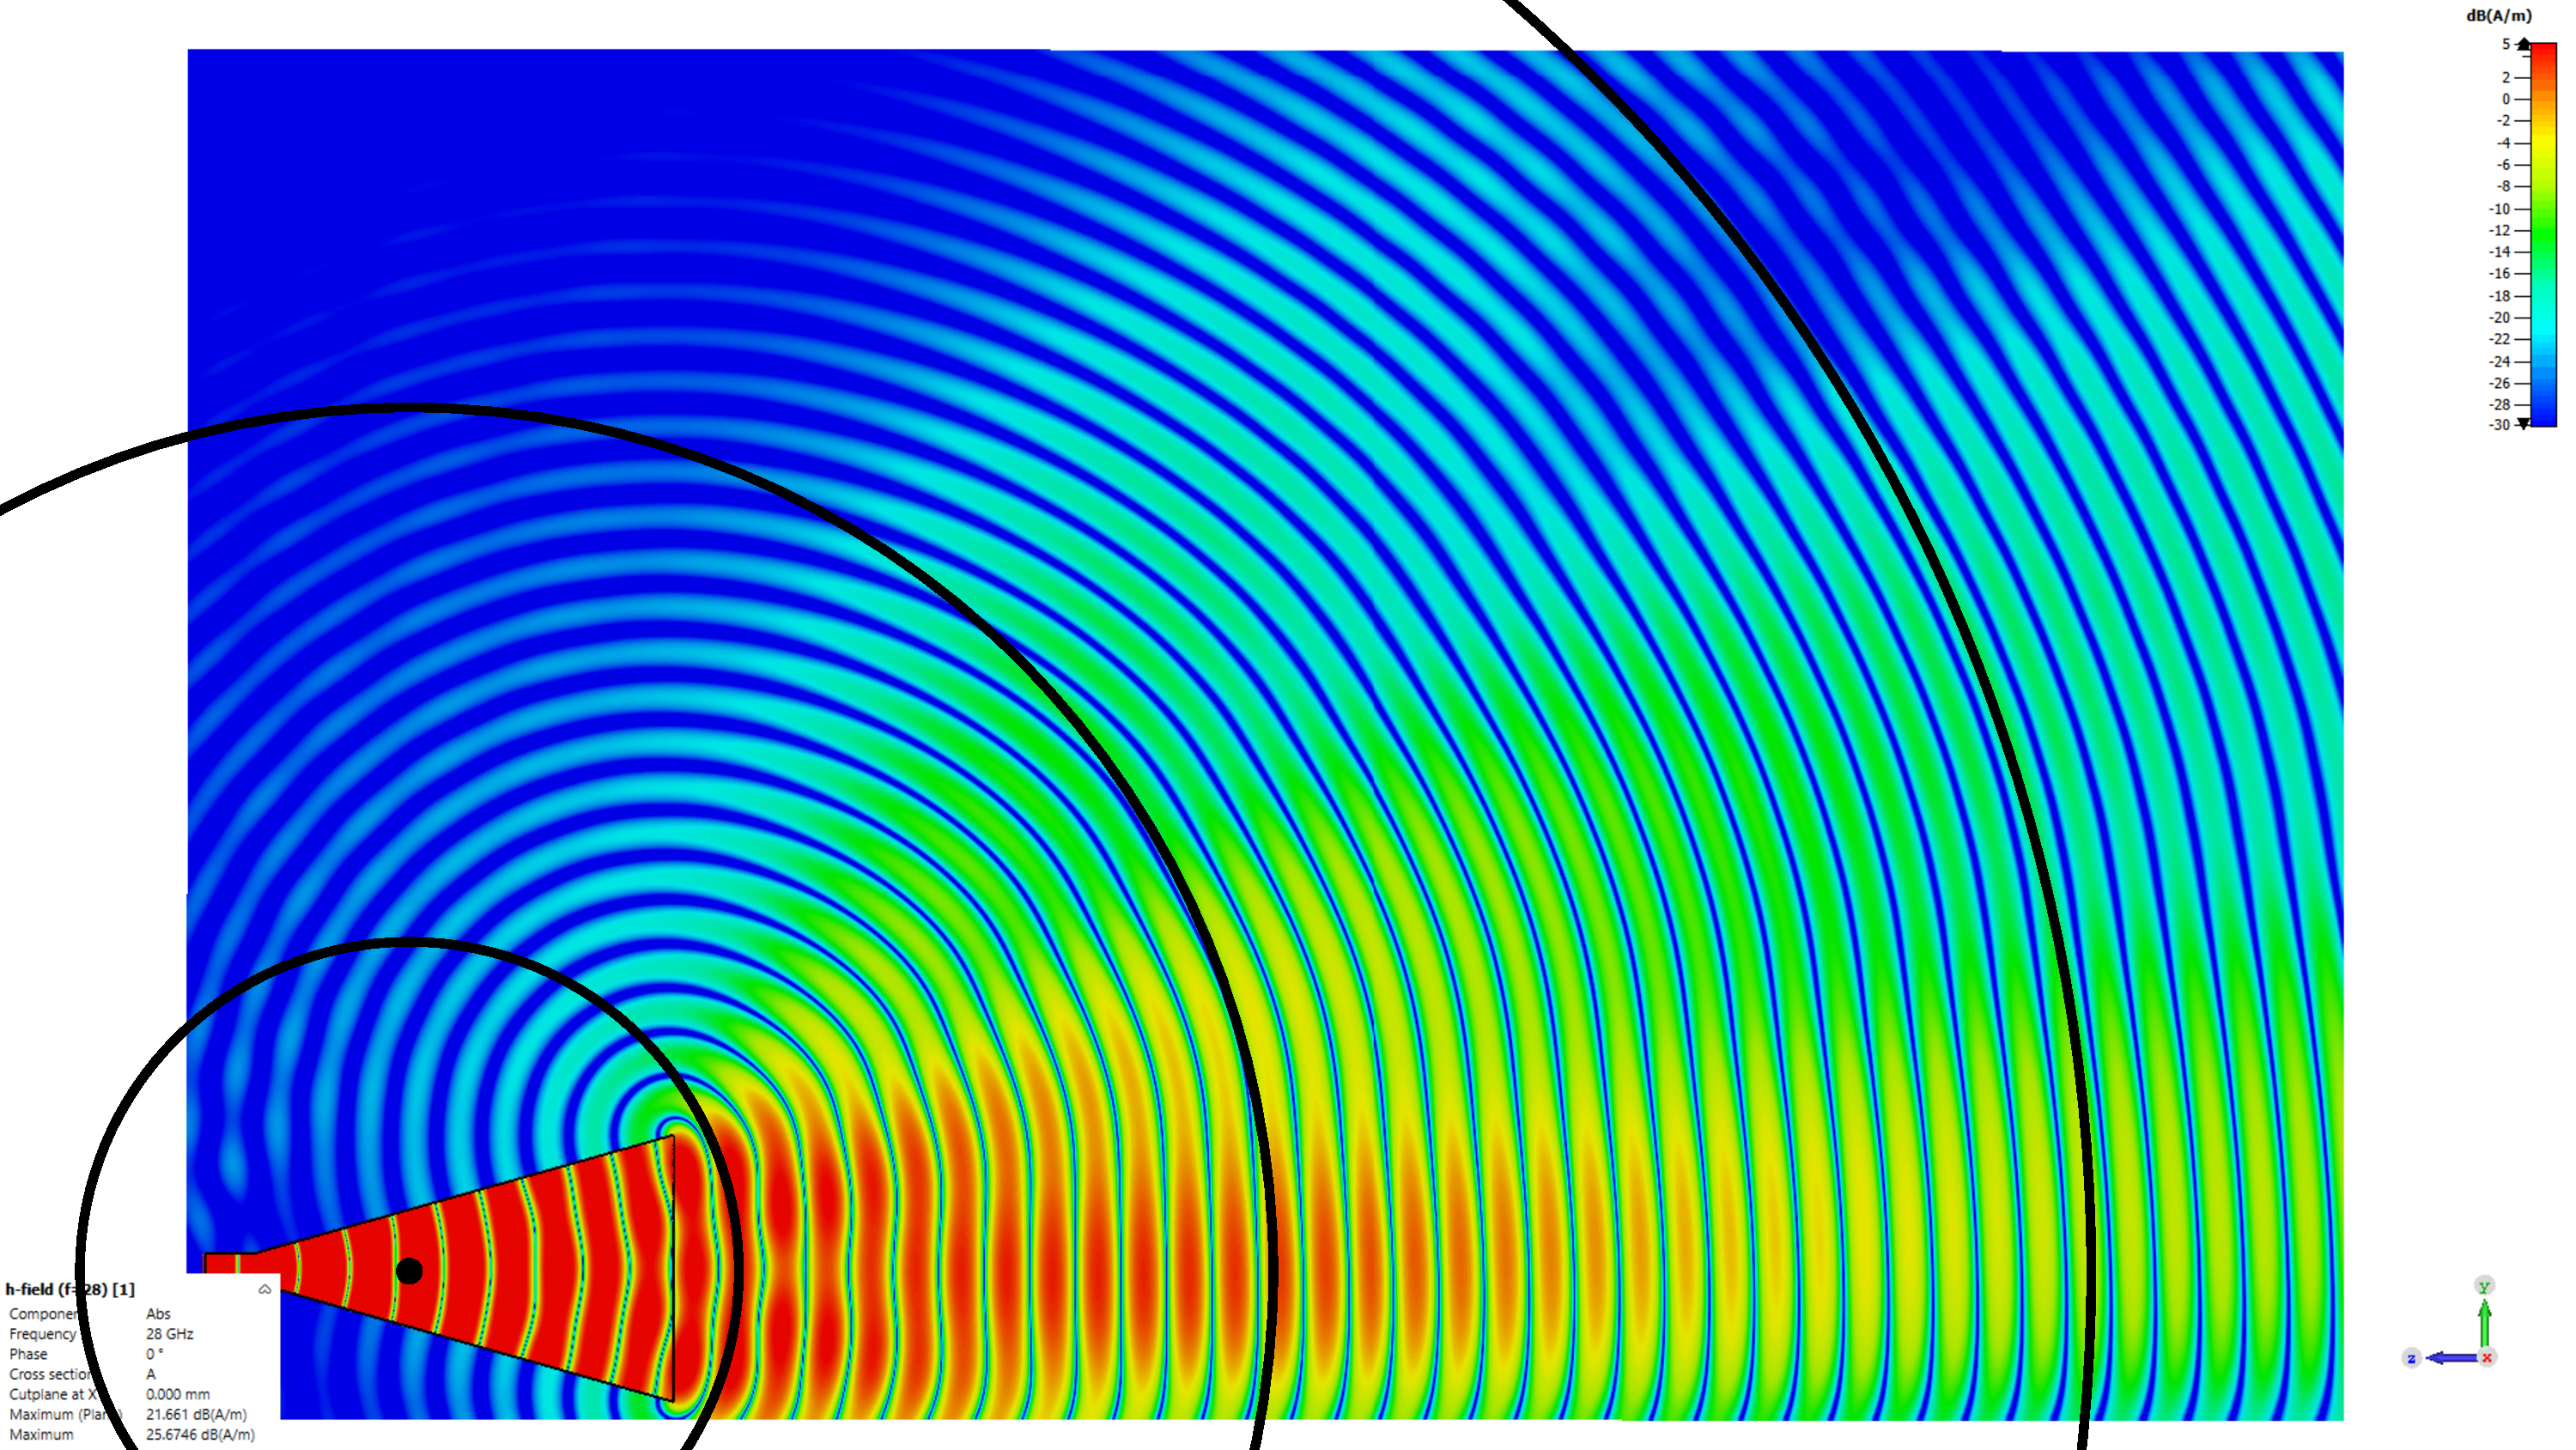
\includegraphics[width=1.5\textwidth , angle=90]{Horn-hf-Field-Region.pdf}
\caption{H-Field of a SGH in E-Plane}
\label{fig:eplaneef}
\end{figure}

\begin{figure}
  \centering
  \subfigure[Cartesian]{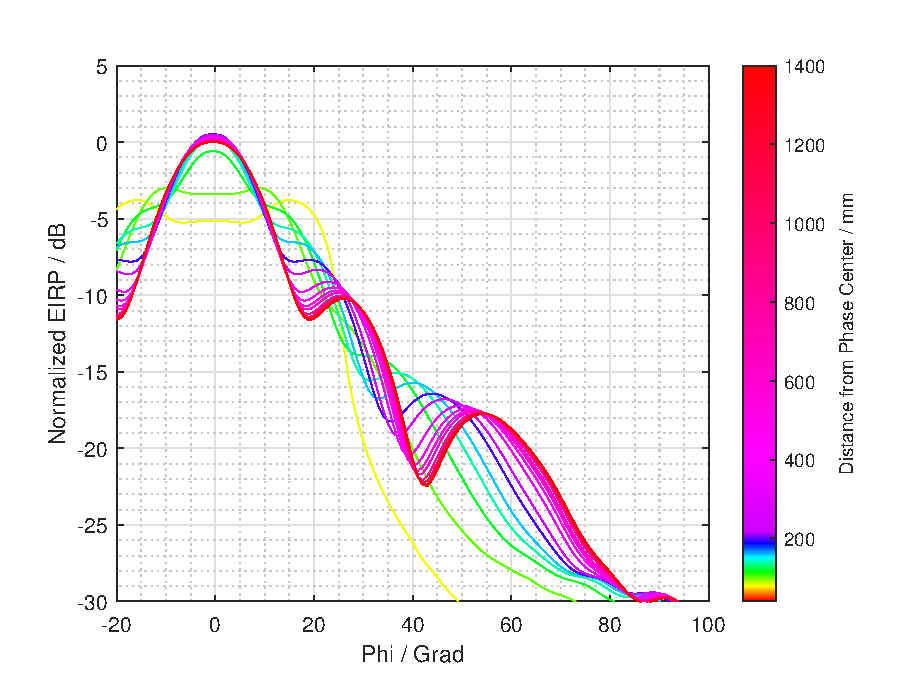
\includegraphics[width=0.8\textwidth]{Matlab/evolvePattern1.eps}}
  \centering
  \subfigure[Polar]{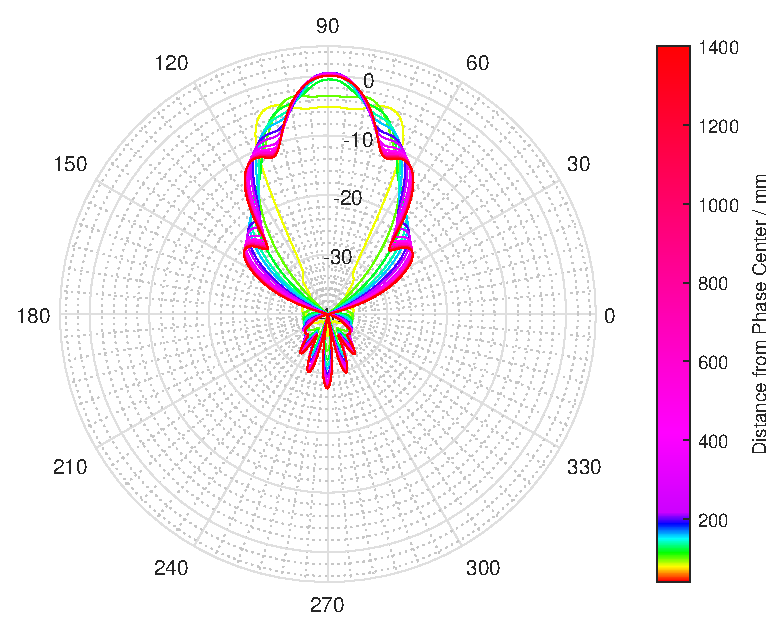
\includegraphics[width=0.8\textwidth]{Matlab/evolvePattern2.eps}}
\caption{Development of the antenna pattern in different radii}
\label{fig:devantennap}
\end{figure}

\begin{figure}
\centering
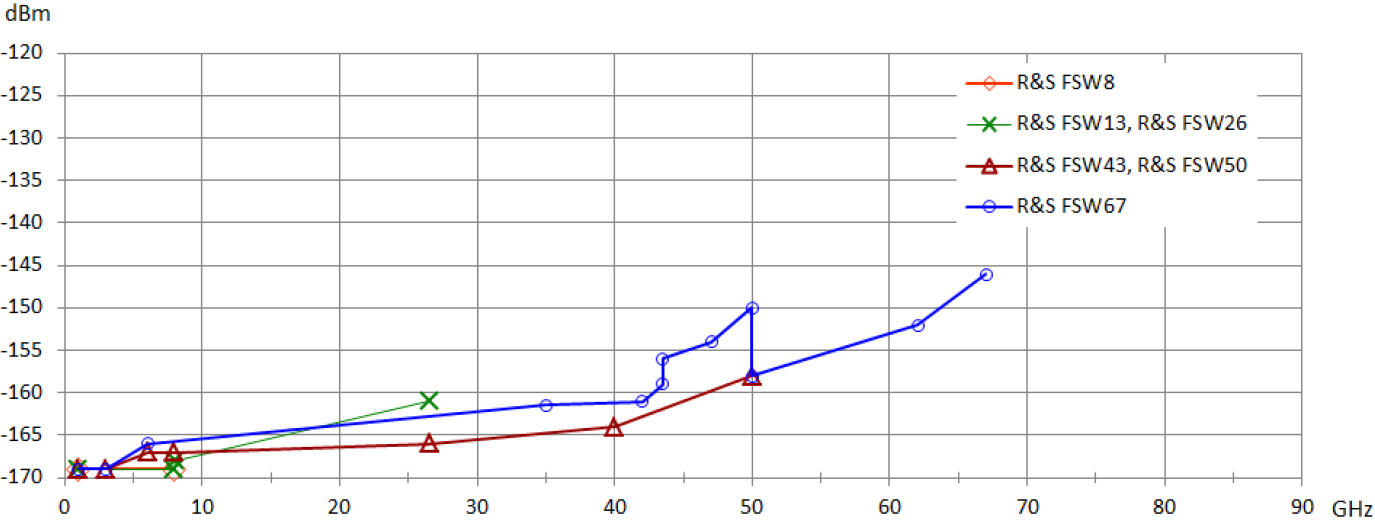
\includegraphics[width=\textwidth]{DANL.png}
\caption{DANL of R\&{}S spectrum analyzers \cite{rsfsw}}
\label{fig:danl}
\end{figure}


\begin{figure}
\centering
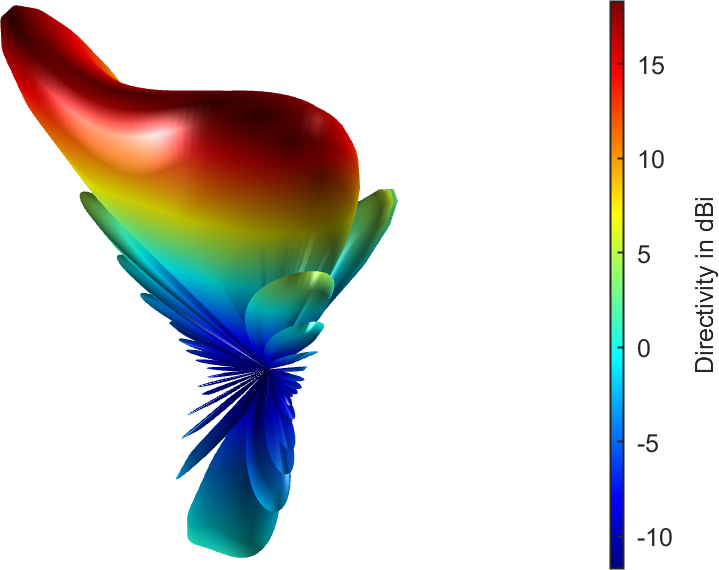
\includegraphics[width=0.4\textwidth]{Matlab/randPattern_3D.png}
\caption{Pattern of a random steering vectors, 6x18-Array}
\label{fig:randp}
\end{figure}


\begin{figure}[h]
  \centering
  \subfigure[Zoom 1]{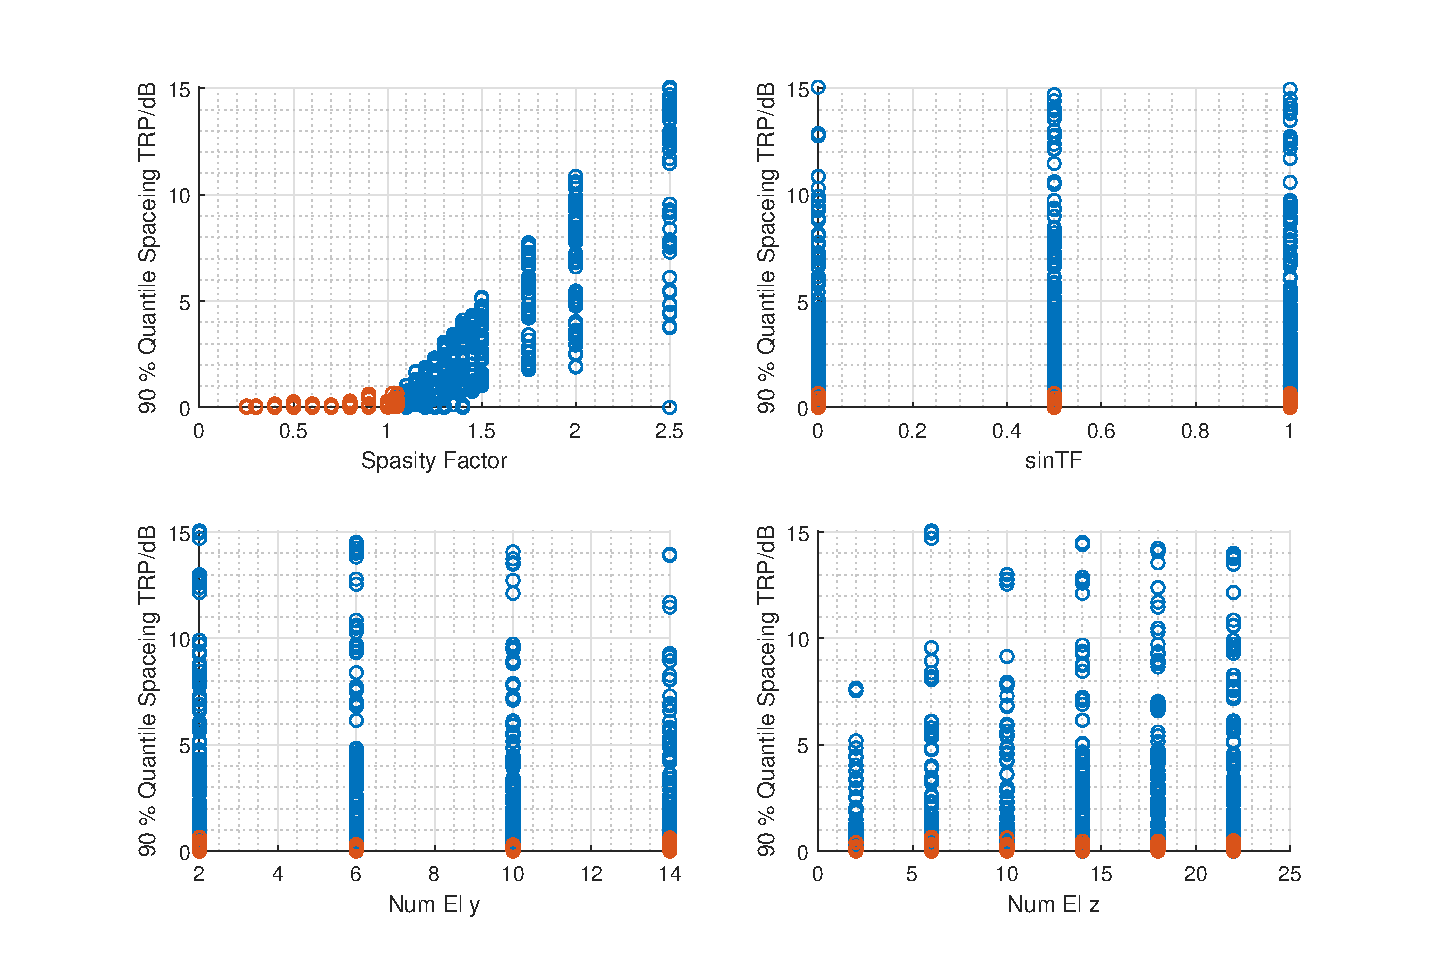
\includegraphics[width=0.9\textwidth]{Matlab/spars-sim4.eps}}
  \centering
  \subfigure[Zoom 2]{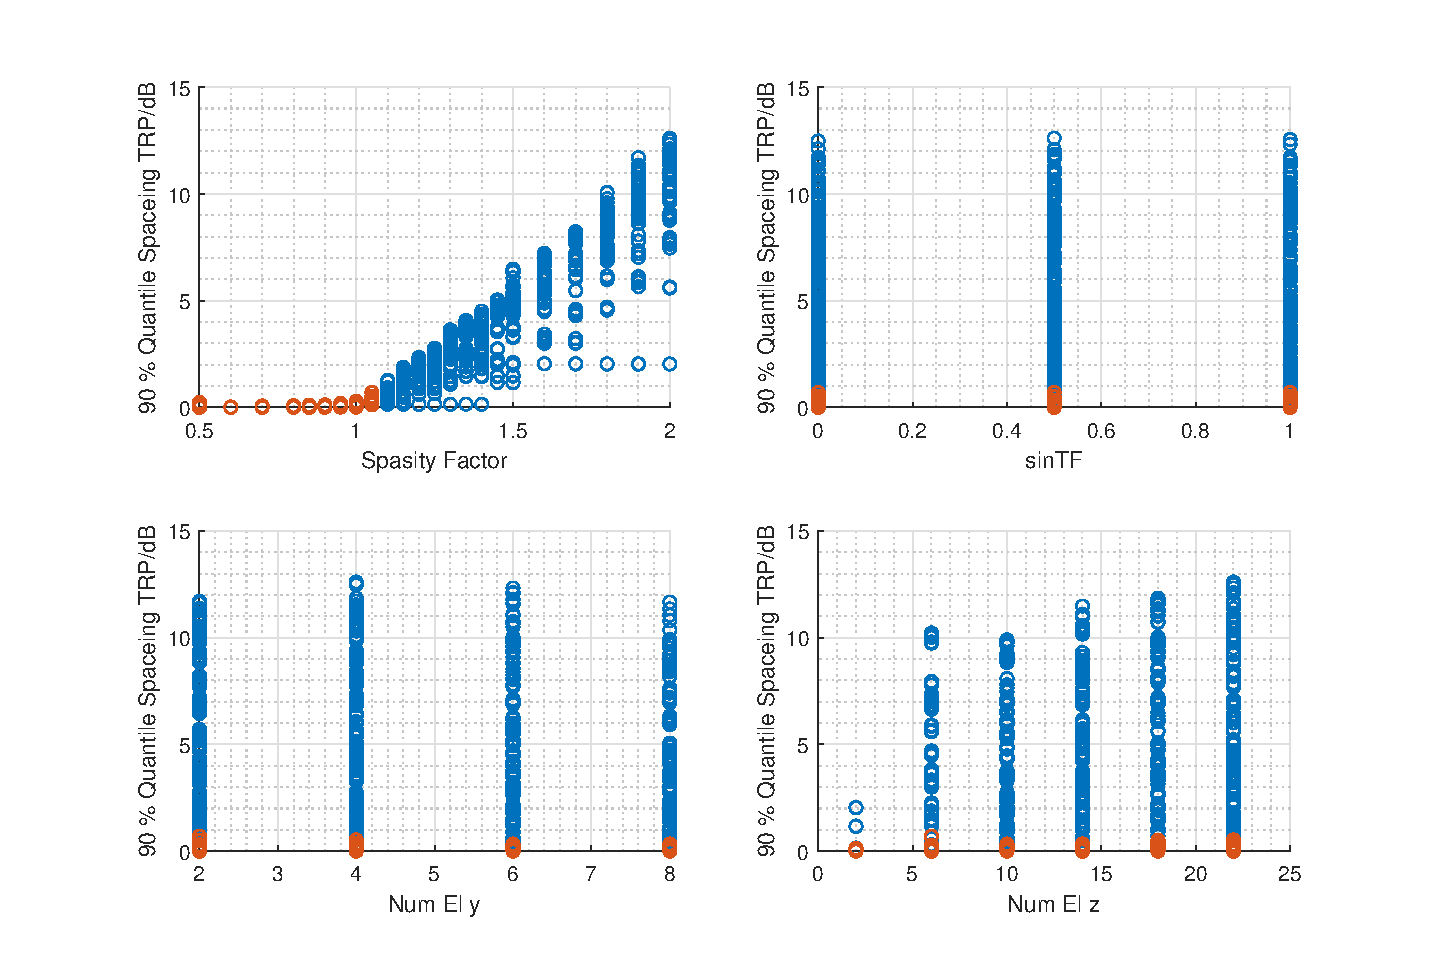
\includegraphics[width=0.9\textwidth]{{Matlab/spars-sim5.eps}}}
\caption{Marginal Probability Sparsity Simulation,IQR , scatter plot}
\label{fig:sparssim3}
\end{figure}

\begin{figure}[h]
  \centering
  \subfigure[Zoom 1]{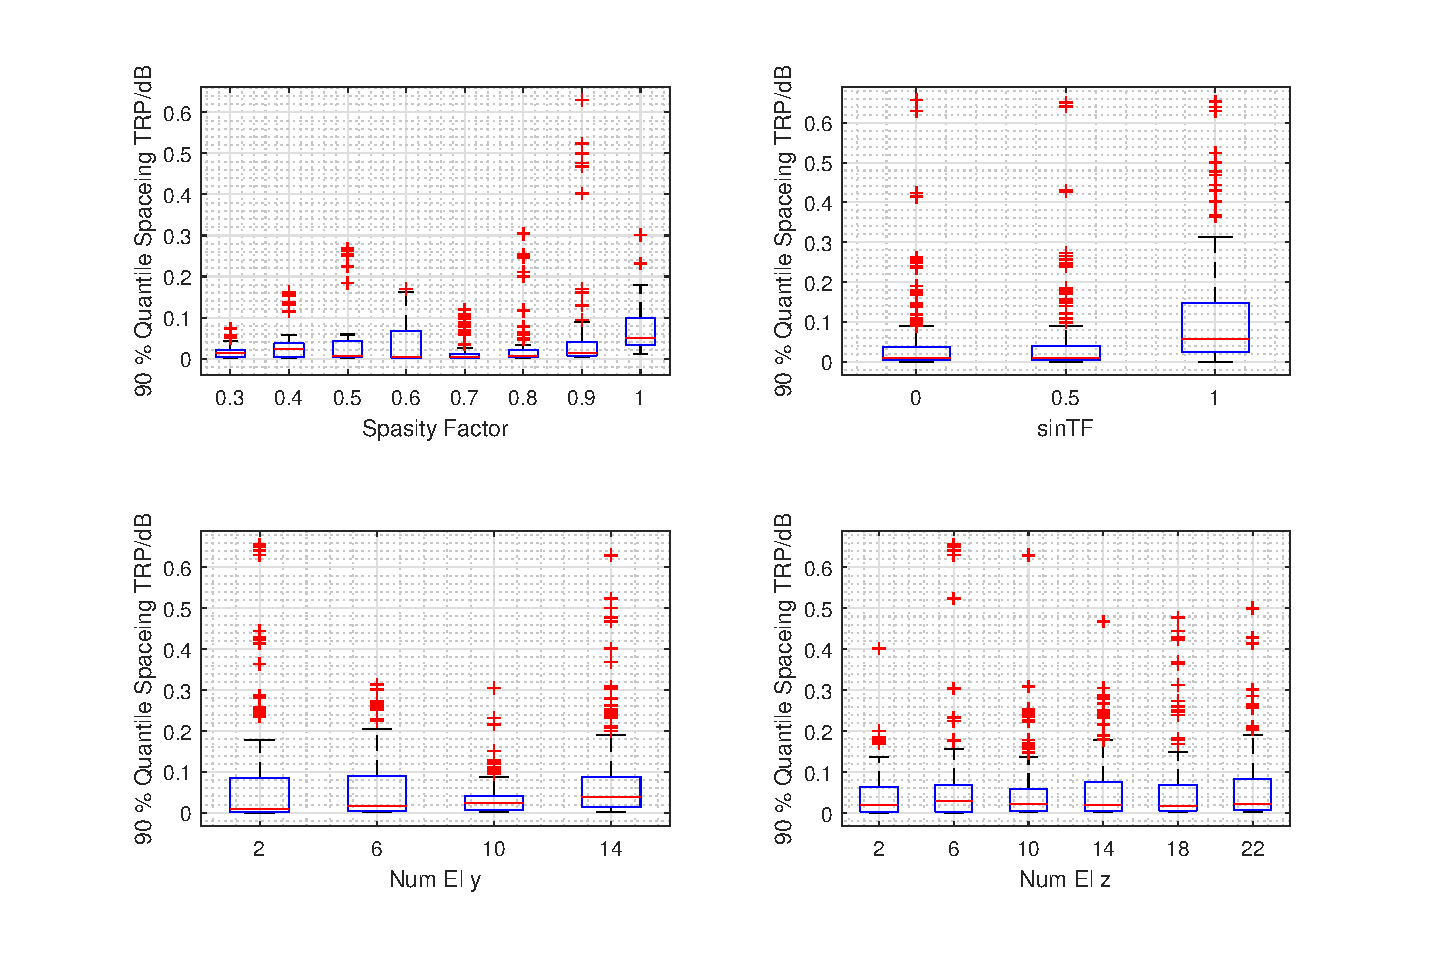
\includegraphics[width=0.9\textwidth]{Matlab/spars-sim-gr-box1.eps}}
  \centering
  \subfigure[Zoom 2]{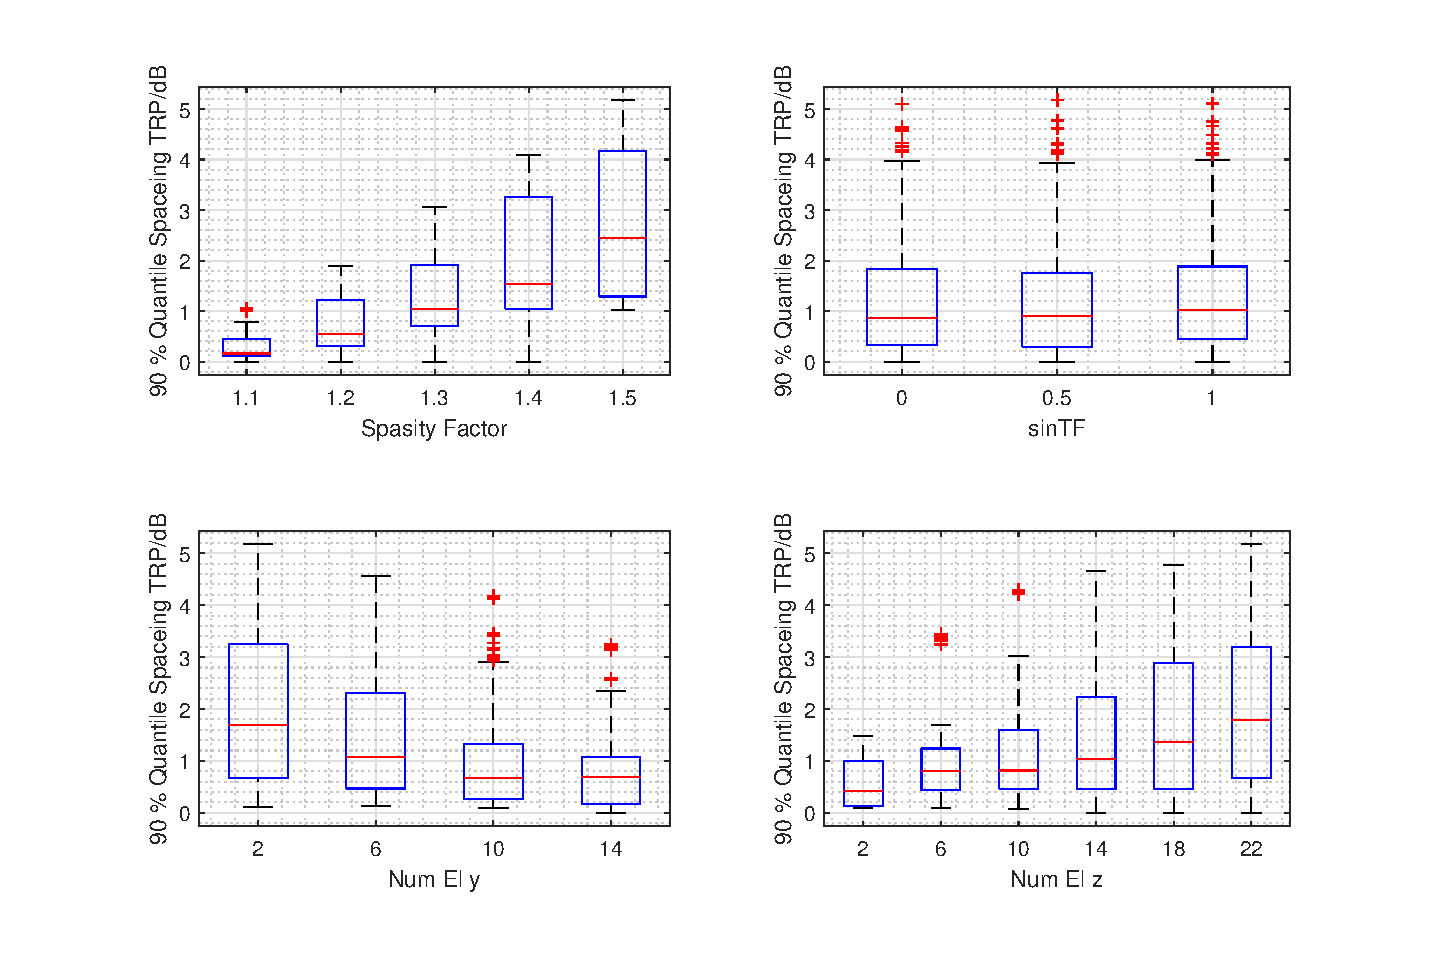
\includegraphics[width=0.9\textwidth]{{Matlab/spars-sim-gr-box2.eps}}}
\caption{Marginal Probability Sparsity Simulation, IQR, box plot}
\label{fig:sparssimbox}
\end{figure}

\begin{figure}[h]
  \centering
  \subfigure[Zoom 1]{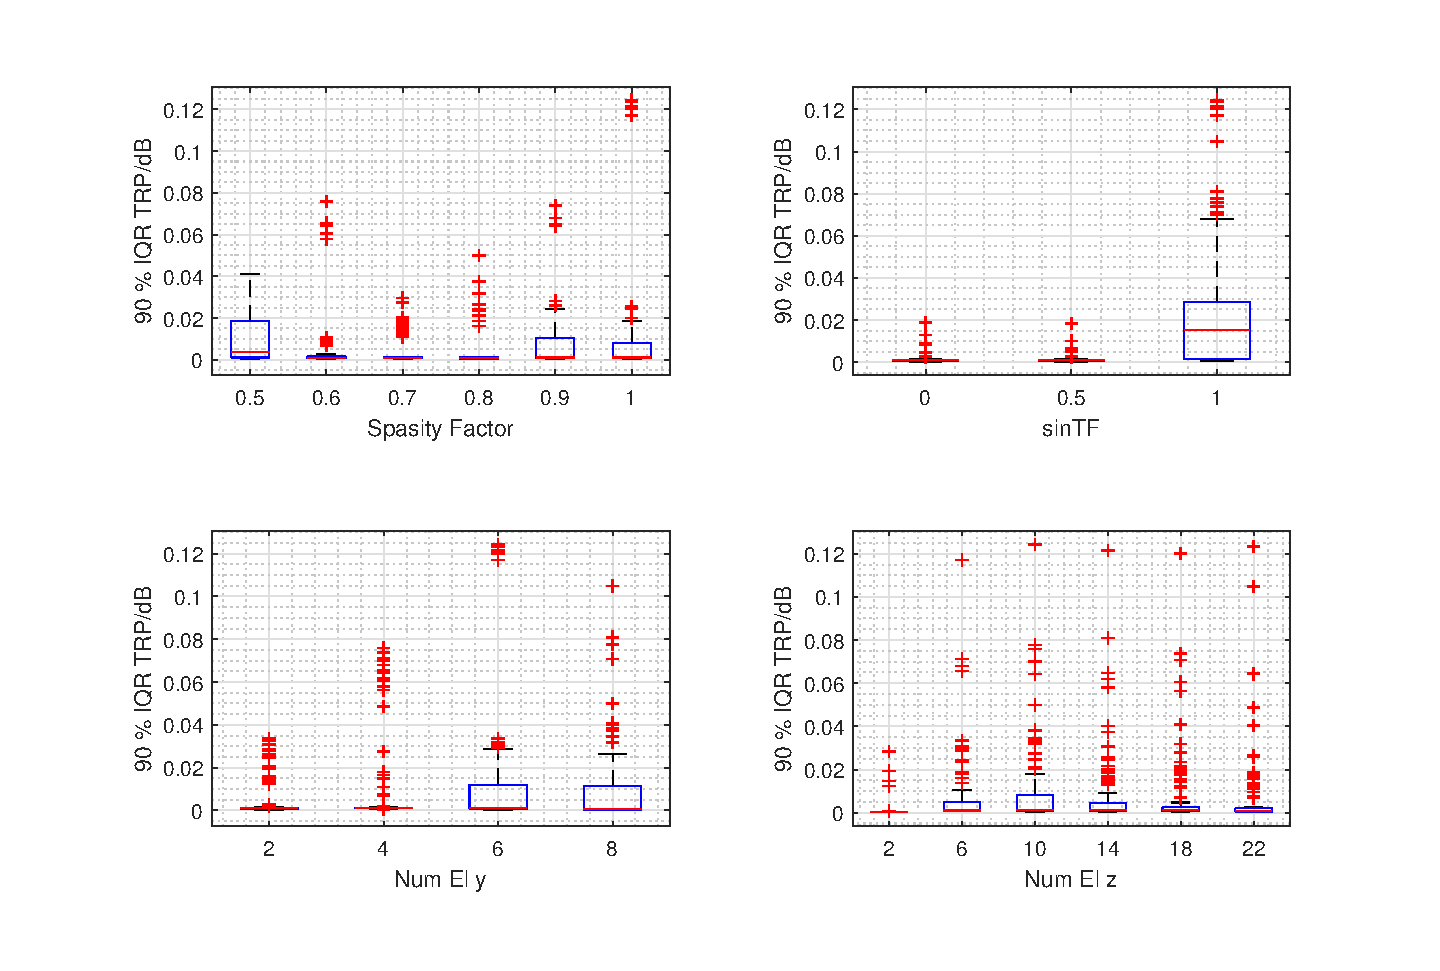
\includegraphics[width=0.9\textwidth]{Matlab/spars-sim-gr-box1-HansenA.eps}}
  \centering
  \subfigure[Zoom 2]{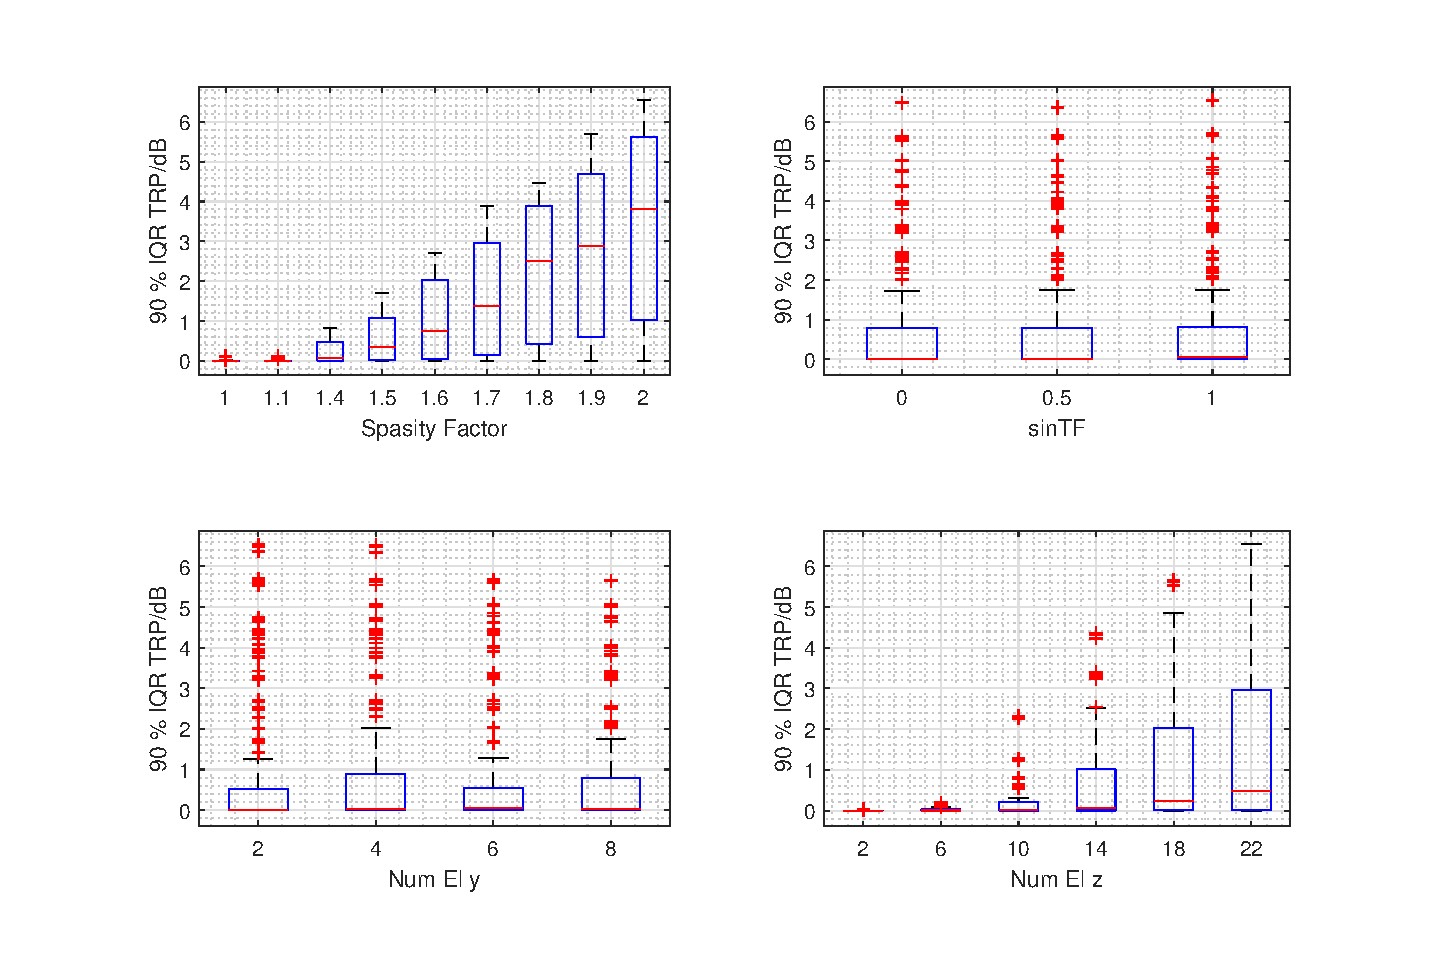
\includegraphics[width=0.9\textwidth]{{Matlab/spars-sim-gr-box2-HansenA.eps}}}
\caption{Marginal Probability Sparsity Simulation, Hansen Angle, IQR, box plot}
\label{fig:sparssimboxhansen}
\end{figure}

\begin{figure}[h]
  \centering
  \subfigure[Zoom 1]{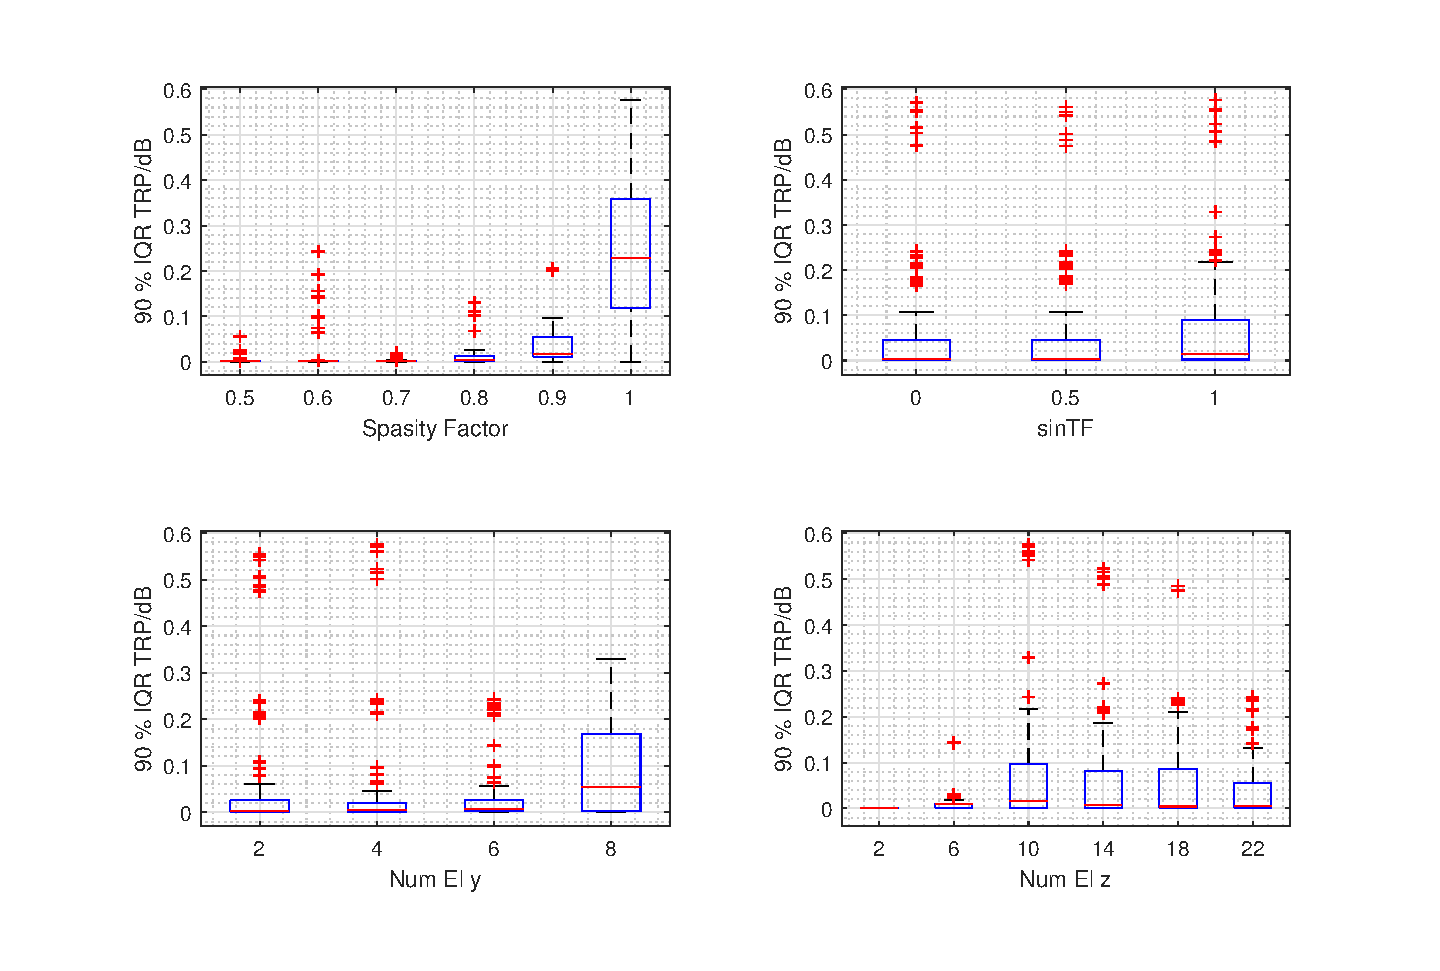
\includegraphics[width=0.9\textwidth]{Matlab/spars-sim-gr-box1-EricssonA.eps}}
  \centering
  \subfigure[Zoom 2]{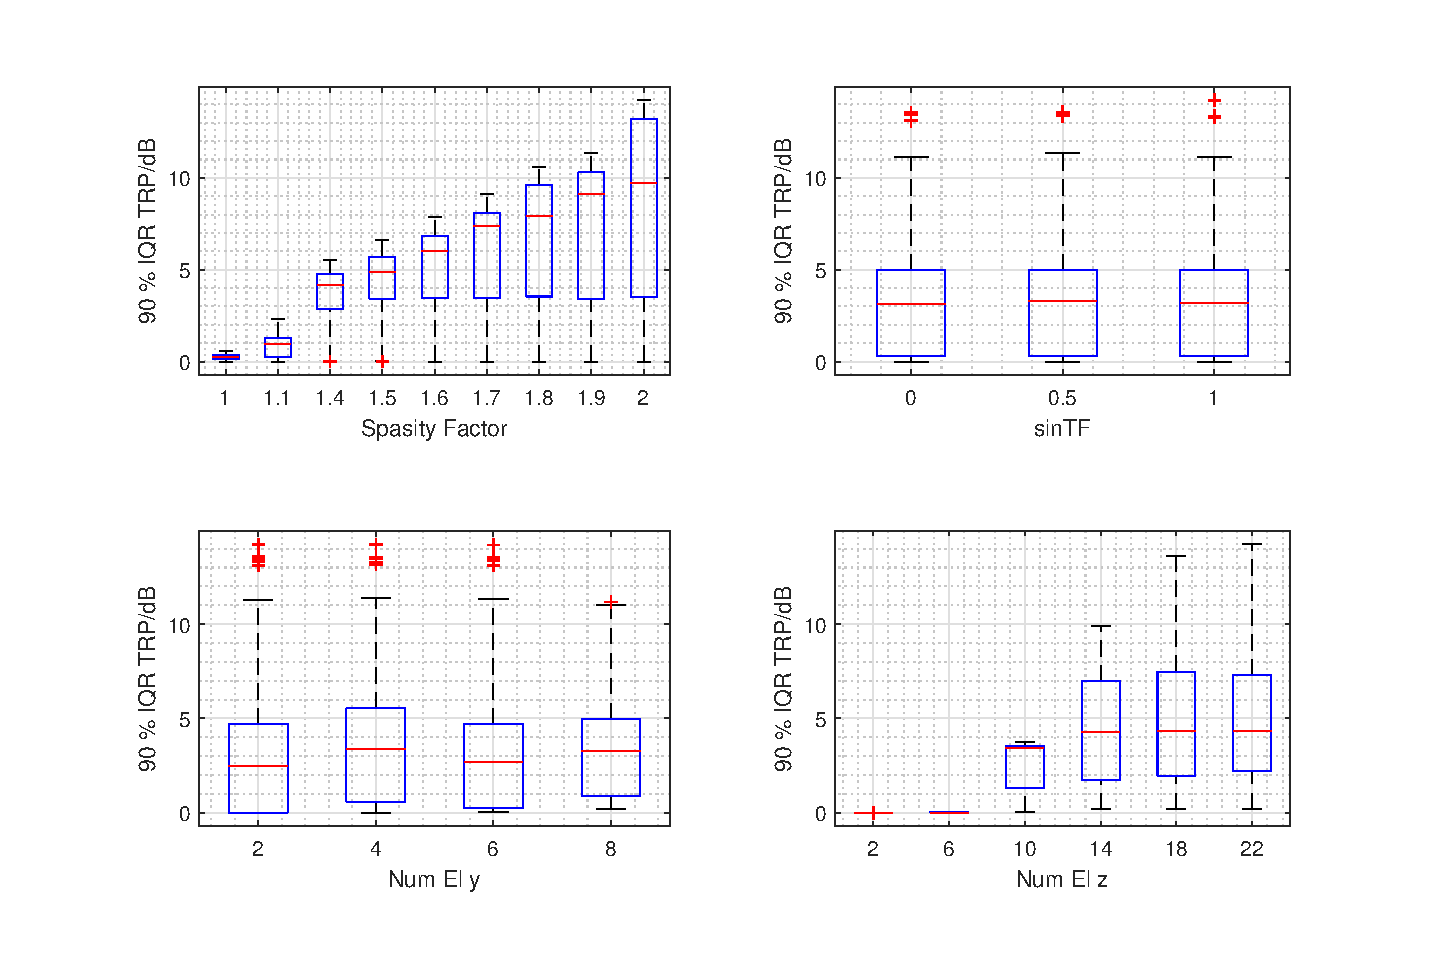
\includegraphics[width=0.9\textwidth]{{Matlab/spars-sim-gr-box2-EricssonA.eps}}}
\caption{Marginal Probability Sparsity Simulation, Ericsson Angle, IQR, box plot}
\label{fig:sparssimboxericsson}
\end{figure}

\begin{figure}[h]
  \centering
  \subfigure[Zoom 1]{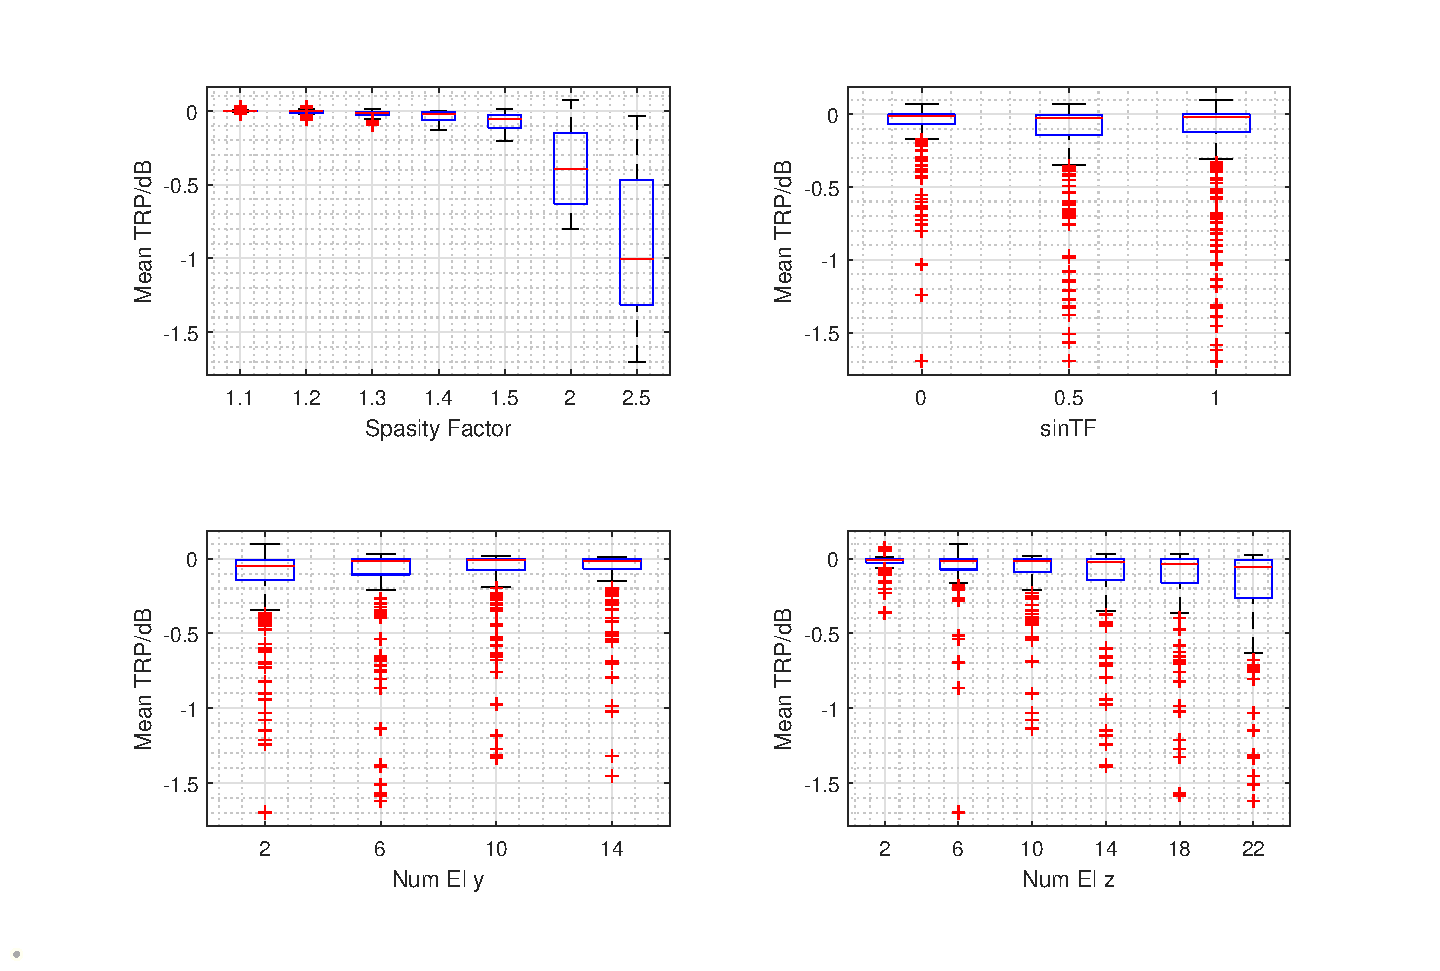
\includegraphics[width=0.9\textwidth]{Matlab/spars-sim-gr-mean-box1.eps}}
  \centering
  \subfigure[Zoom 2]{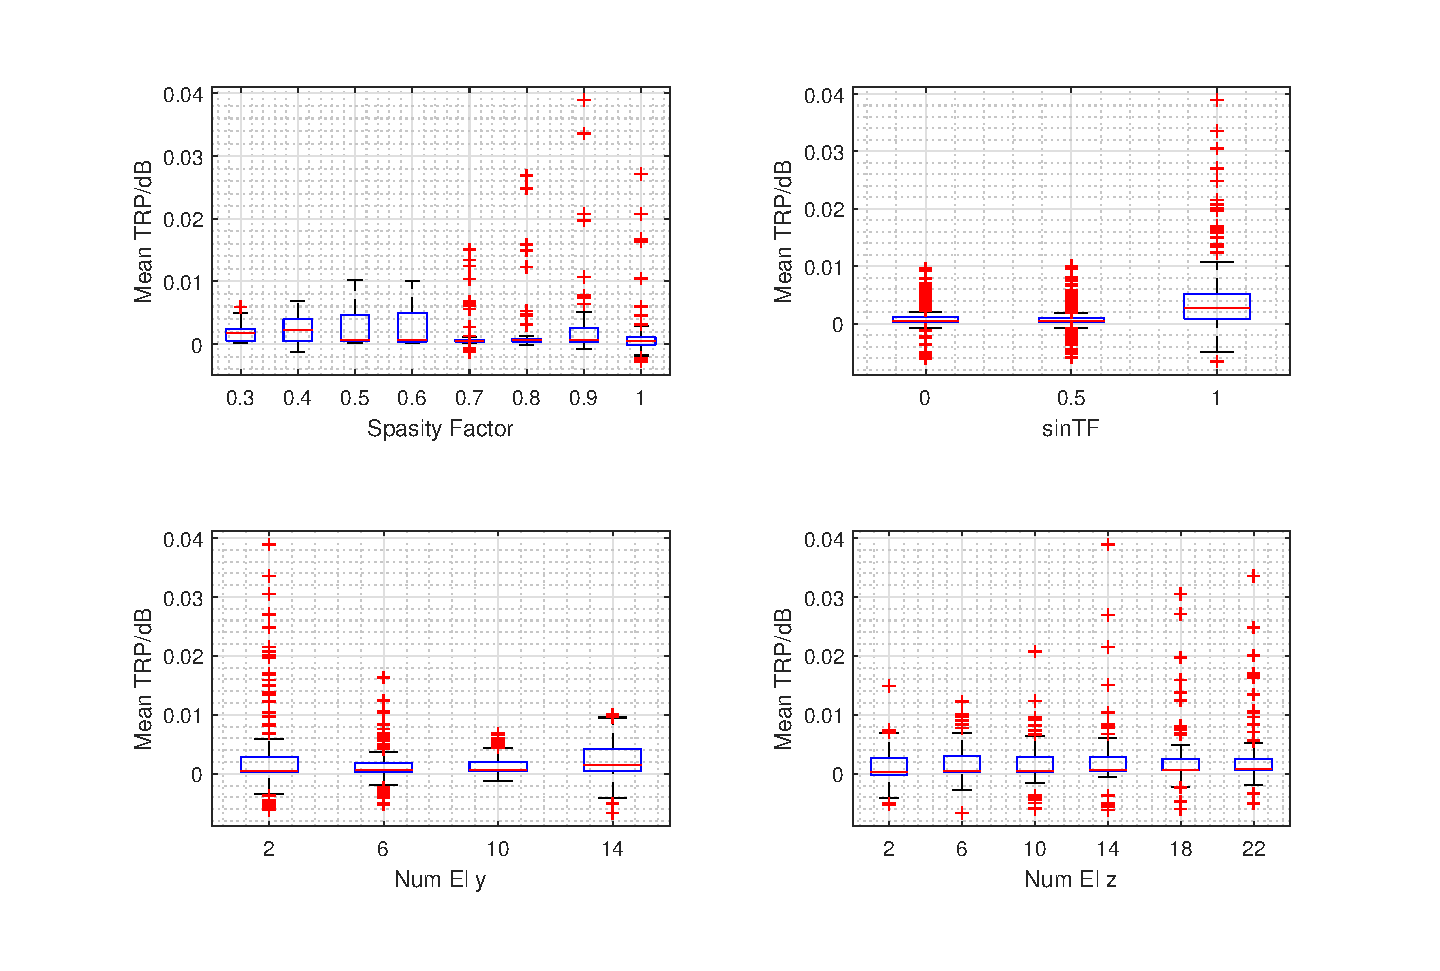
\includegraphics[width=0.9\textwidth]{{Matlab/spars-sim-gr-mean-box2.eps}}}
\caption{Marginal Probability Sparsity Simulation, mean,  box plot}
\label{fig:sparssimboxmean}
\end{figure}

\begin{figure}[h]
  \centering
  \subfigure[Measurement Radius $\SI{8}{\centi\meter}$]{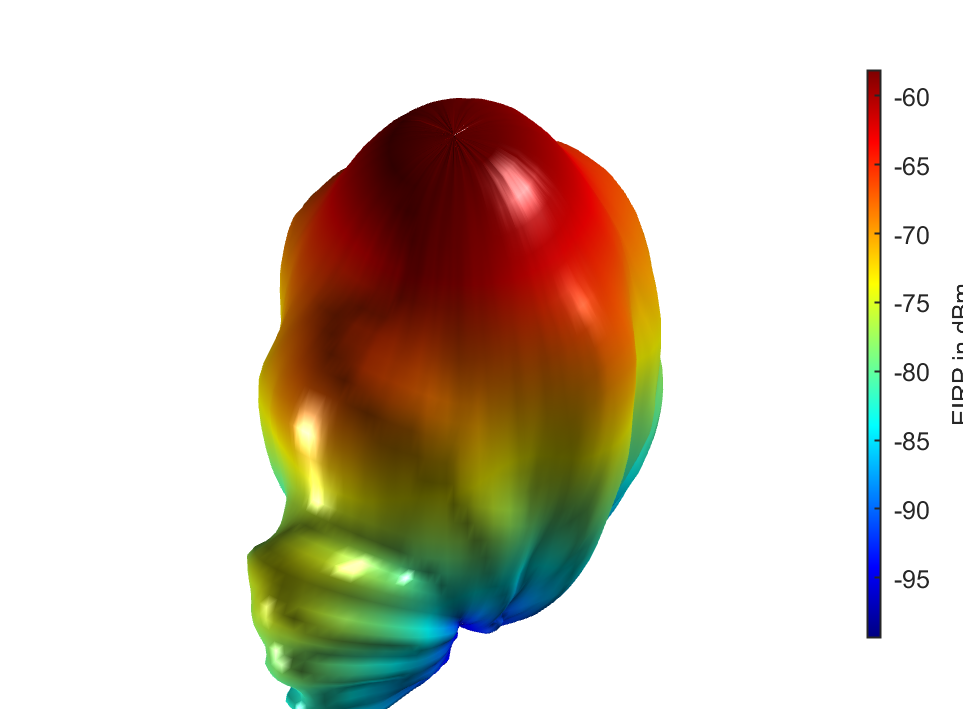
\includegraphics[width=0.32\textwidth]{Pattern/OEWG2/Radius008cm_3D.png}}
  \centering
  \subfigure[Measurement Radius $\SI{8.6}{\centi\meter}$]{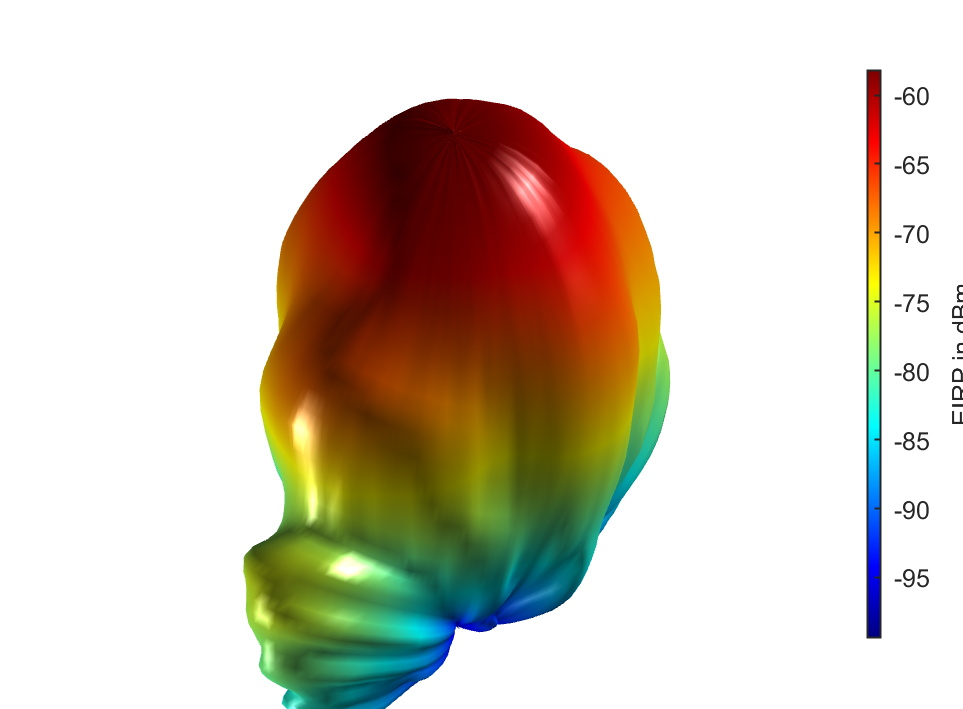
\includegraphics[width=0.32\textwidth]{Pattern/OEWG2/Radius0086cm_3D.png}}
  \centering
  \subfigure[Measurement Radius $\SI{9.6}{\centi\meter}$]{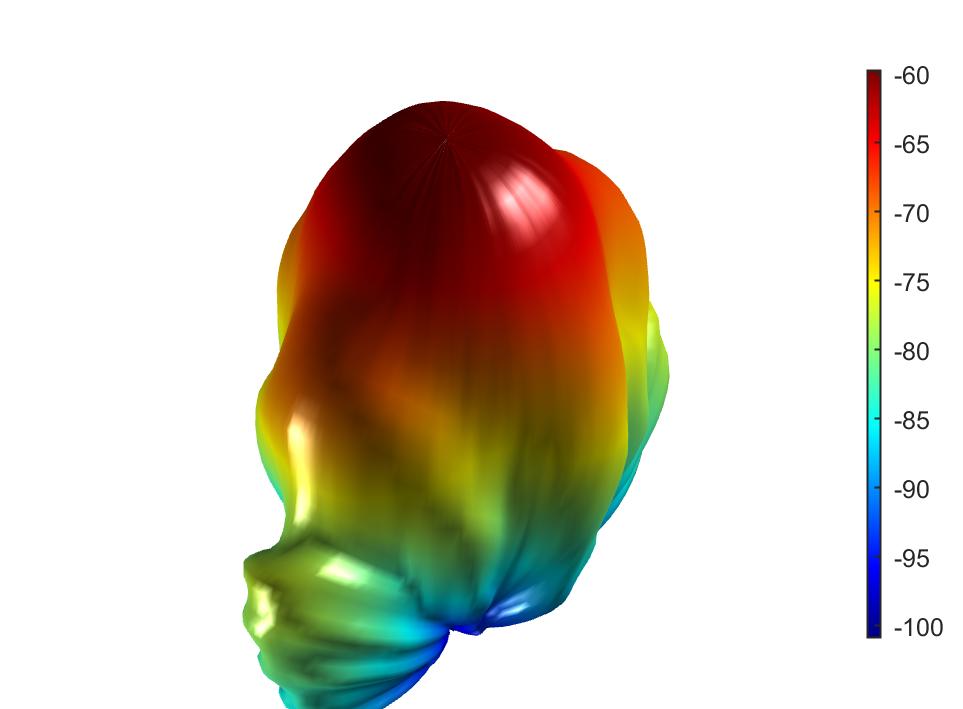
\includegraphics[width=0.32\textwidth]{Pattern/OEWG2/Radius0096cm_3D.png}}
  \centering
  \subfigure[Measurement Radius $\SI{10.6}{\centi\meter}$]{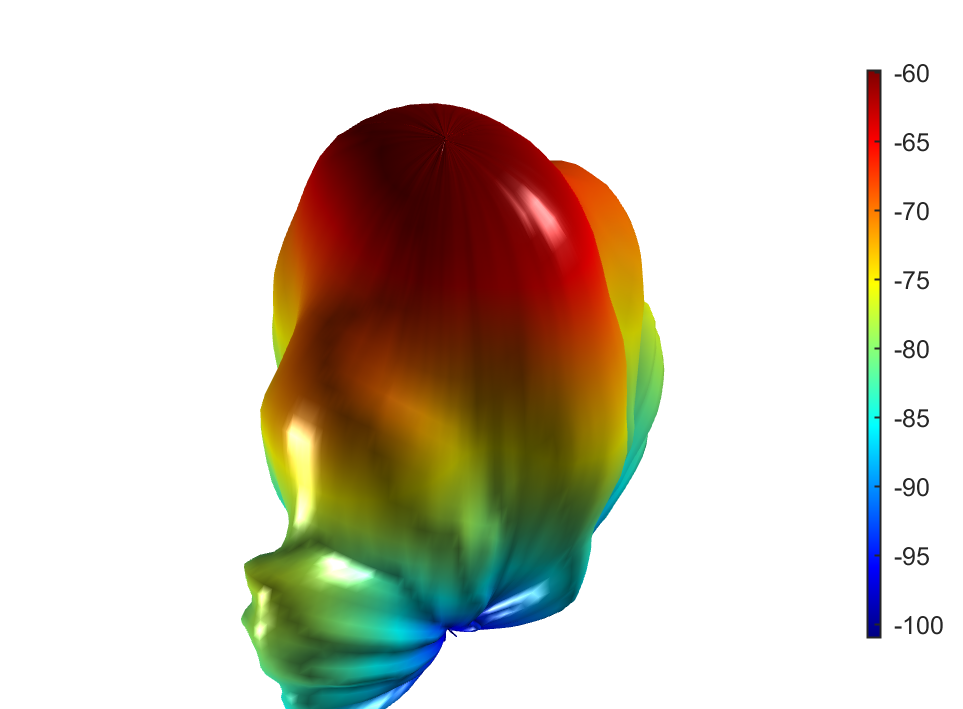
\includegraphics[width=0.32\textwidth]{Pattern/OEWG2/Radius0106cm_3D.png}}
  \centering
  \subfigure[Measurement Radius $\SI{11.6}{\centi\meter}$]{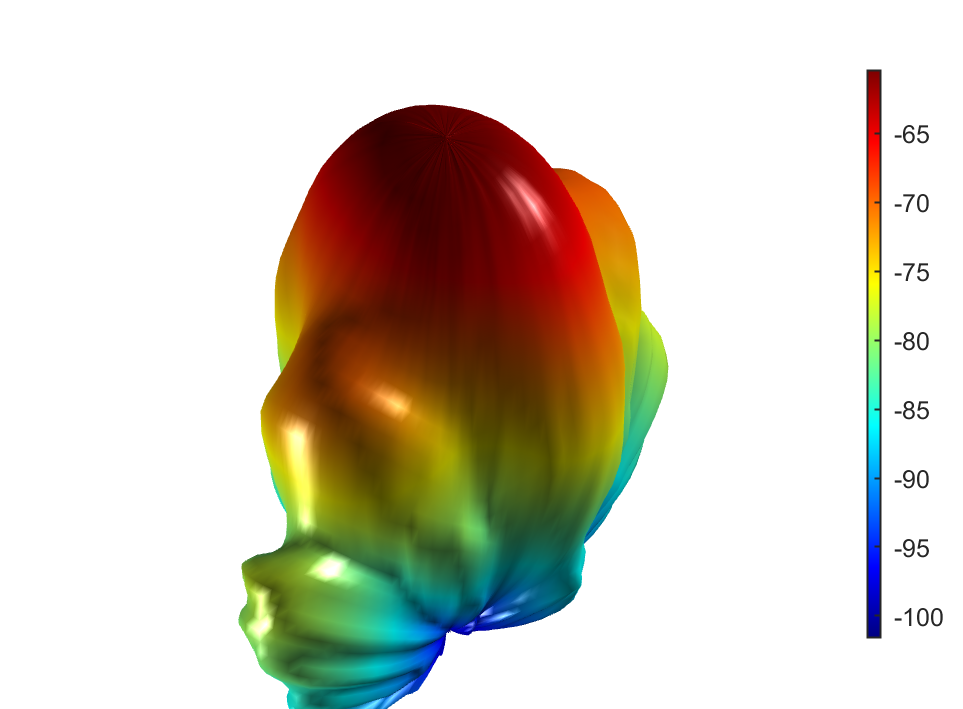
\includegraphics[width=0.32\textwidth]{Pattern/OEWG2/Radius0116cm_3D.png}}
  \centering
  \subfigure[Measurement Radius $\SI{12.6}{\centi\meter}$]{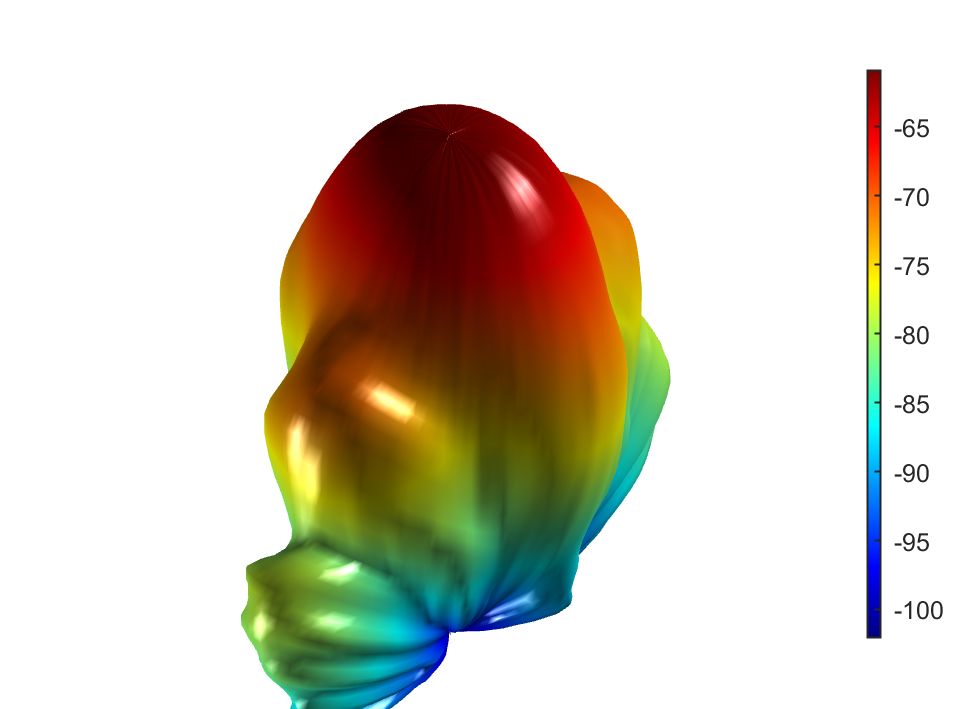
\includegraphics[width=0.32\textwidth]{Pattern/OEWG2/Radius0126cm_3D.png}}
  \centering
  \subfigure[Measurement Radius $\SI{13.6}{\centi\meter}$]{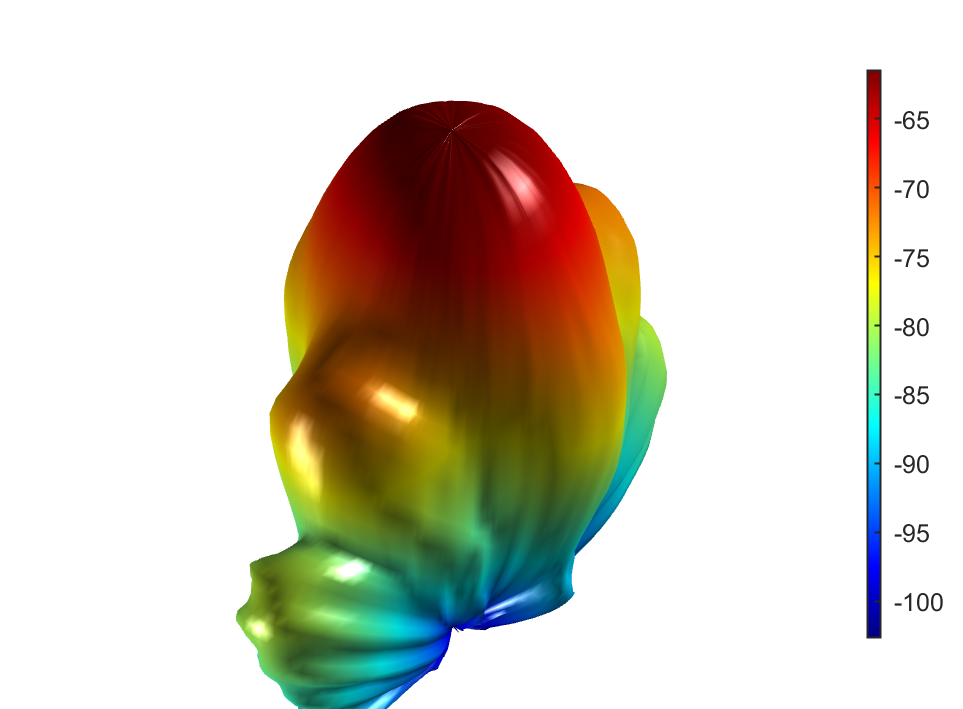
\includegraphics[width=0.32\textwidth]{Pattern/OEWG2/Radius0136cm_3D.png}}
  \centering
  \subfigure[Measurement Radius $\SI{14.6}{\centi\meter}$]{\includegraphics[width=0.32\textwidth]{Pattern/OEWG2/Radius0146cm_3D.png}}
  \centering
  \subfigure[Measurement Radius $\SI{15.6}{\centi\meter}$]{\includegraphics[width=0.32\textwidth]{Pattern/OEWG2/Radius0156cm_3D.png}}
  \centering
  \subfigure[Measurement Radius $\SI{16.6}{\centi\meter}$]{\includegraphics[width=0.32\textwidth]{Pattern/OEWG2/Radius0166cm_3D.png}}
  \centering
  \subfigure[Measurement Radius $\SI{18.6}{\centi\meter}$]{\includegraphics[width=0.32\textwidth]{Pattern/OEWG2/Radius0186cm_3D.png}}
  \centering
  \subfigure[Measurement Radius $\SI{23.6}{\centi\meter}$]{\includegraphics[width=0.32\textwidth]{Pattern/OEWG2/Radius0236cm_3D.png}}
\caption{Measured SGH Antenna-EIRP Pattern with OEWG 2 Probe in different Radii}
\label{fig:sghpatternoewg2}
\end{figure}


\begin{figure}[h]
  \centering
  \subfigure[Measurement Radius $\SI{15.2}{\centi\meter}$]{\includegraphics[width=0.32\textwidth]{Pattern/Patch/Radius0152cm_3D.png}}
  \centering
  \subfigure[Measurement Radius $\SI{15.7}{\centi\meter}$]{\includegraphics[width=0.32\textwidth]{Pattern/Patch/Radius0157cm_3D.png}}
  \centering
  \subfigure[Measurement Radius $\SI{16.7}{\centi\meter}$]{\includegraphics[width=0.32\textwidth]{Pattern/Patch/Radius0167cm_3D.png}}
  \centering
  \subfigure[Measurement Radius $\SI{17.7}{\centi\meter}$]{\includegraphics[width=0.32\textwidth]{Pattern/Patch/Radius0177cm_3D.png}}
  \centering
  \subfigure[Measurement Radius $\SI{19.7}{\centi\meter}$]{\includegraphics[width=0.32\textwidth]{Pattern/Patch/Radius0197cm_3D.png}}
  \centering
  \subfigure[Measurement Radius $\SI{21.7}{\centi\meter}$]{\includegraphics[width=0.32\textwidth]{Pattern/Patch/Radius0217cm_3D.png}}
  \centering
  \subfigure[Measurement Radius $\SI{23.7}{\centi\meter}$]{\includegraphics[width=0.32\textwidth]{Pattern/Patch/Radius0237cm_3D.png}}
  \centering
  \subfigure[Measurement Radius $\SI{25.7}{\centi\meter}$]{\includegraphics[width=0.32\textwidth]{Pattern/Patch/Radius0257cm_3D.png}}
  \centering
  \subfigure[Measurement Radius $\SI{30.7}{\centi\meter}$]{\includegraphics[width=0.32\textwidth]{Pattern/Patch/Radius0307cm_3D.png}}
  \centering
  \subfigure[Measurement Radius $\SI{35.7}{\centi\meter}$]{\includegraphics[width=0.32\textwidth]{Pattern/Patch/Radius0357cm_3D.png}}
  \centering
  \subfigure[Measurement Radius $\SI{40.7}{\centi\meter}$]{\includegraphics[width=0.32\textwidth]{Pattern/Patch/Radius0407cm_3D.png}}
  \centering
  \subfigure[Measurement Radius $\SI{45.7}{\centi\meter}$]{\includegraphics[width=0.32\textwidth]{Pattern/Patch/Radius0457cm_3D.png}}
\caption{Measured SGH Antenna-EIRP Pattern with Patch Probe in different Radii}
\label{fig:sghpatternpatch}
\end{figure}

\begin{figure}[h]
  \centering
  \subfigure[Measurement Radius $\SI{5}{\centi\meter}$]{\includegraphics[width=0.32\textwidth]{Pattern/Vivaldi/Radius05cm_3D.png}}
  \centering
  \subfigure[Measurement Radius $\SI{13}{\centi\meter}$]{\includegraphics[width=0.32\textwidth]{Pattern/Vivaldi/Radius013cm_3D.png}}
  \centering
  \subfigure[Measurement Radius $\SI{15}{\centi\meter}$]{\includegraphics[width=0.32\textwidth]{Pattern/Vivaldi/Radius015cm_3D.png}}
  \centering
  \subfigure[Measurement Radius $\SI{17}{\centi\meter}$]{\includegraphics[width=0.32\textwidth]{Pattern/Vivaldi/Radius017cm_3D.png}}
  \centering
  \subfigure[Measurement Radius $\SI{19}{\centi\meter}$]{\includegraphics[width=0.32\textwidth]{Pattern/Vivaldi/Radius019cm_3D.png}}
  \centering
  \subfigure[Measurement Radius $\SI{21}{\centi\meter}$]{\includegraphics[width=0.32\textwidth]{Pattern/Vivaldi/Radius021cm_3D.png}}
  \centering
  \subfigure[Measurement Radius $\SI{23}{\centi\meter}$]{\includegraphics[width=0.32\textwidth]{Pattern/Vivaldi/Radius023cm_3D.png}}
  \centering
  \subfigure[Measurement Radius $\SI{25}{\centi\meter}$]{\includegraphics[width=0.32\textwidth]{Pattern/Vivaldi/Radius025cm_3D.png}}
  \centering
  \subfigure[Measurement Radius $\SI{27}{\centi\meter}$]{\includegraphics[width=0.32\textwidth]{Pattern/Vivaldi/Radius027cm_3D.png}}
  \centering
  \subfigure[Measurement Radius $\SI{29}{\centi\meter}$]{\includegraphics[width=0.32\textwidth]{Pattern/Vivaldi/Radius029cm_3D.png}}
  \centering
  \subfigure[Measurement Radius $\SI{31}{\centi\meter}$]{\includegraphics[width=0.32\textwidth]{Pattern/Vivaldi/Radius031cm_3D.png}}
  \centering
  \subfigure[Measurement Radius $\SI{33}{\centi\meter}$]{\includegraphics[width=0.32\textwidth]{Pattern/Vivaldi/Radius033cm_3D.png}}
\caption{Measured SGH Antenna-EIRP Pattern with Vivaldi Probe in different Radii}
\label{fig:sghpatternvivaldi}
\end{figure}
